\documentclass[twoside]{book}

% Packages required by doxygen
\usepackage{fixltx2e}
\usepackage{calc}
\usepackage{doxygen}
\usepackage[export]{adjustbox} % also loads graphicx
\usepackage{graphicx}
\usepackage[utf8]{inputenc}
\usepackage{makeidx}
\usepackage{multicol}
\usepackage{multirow}
\PassOptionsToPackage{warn}{textcomp}
\usepackage{textcomp}
\usepackage[nointegrals]{wasysym}
\usepackage[table]{xcolor}

% Font selection
\usepackage[T1]{fontenc}
\usepackage[scaled=.90]{helvet}
\usepackage{courier}
\usepackage{amssymb}
\usepackage{sectsty}
\renewcommand{\familydefault}{\sfdefault}
\allsectionsfont{%
  \fontseries{bc}\selectfont%
  \color{darkgray}%
}
\renewcommand{\DoxyLabelFont}{%
  \fontseries{bc}\selectfont%
  \color{darkgray}%
}
\newcommand{\+}{\discretionary{\mbox{\scriptsize$\hookleftarrow$}}{}{}}

% Page & text layout
\usepackage{geometry}
\geometry{%
  a4paper,%
  top=2.5cm,%
  bottom=2.5cm,%
  left=2.5cm,%
  right=2.5cm%
}
\tolerance=750
\hfuzz=15pt
\hbadness=750
\setlength{\emergencystretch}{15pt}
\setlength{\parindent}{0cm}
\setlength{\parskip}{3ex plus 2ex minus 2ex}
\makeatletter
\renewcommand{\paragraph}{%
  \@startsection{paragraph}{4}{0ex}{-1.0ex}{1.0ex}{%
    \normalfont\normalsize\bfseries\SS@parafont%
  }%
}
\renewcommand{\subparagraph}{%
  \@startsection{subparagraph}{5}{0ex}{-1.0ex}{1.0ex}{%
    \normalfont\normalsize\bfseries\SS@subparafont%
  }%
}
\makeatother

% Headers & footers
\usepackage{fancyhdr}
\pagestyle{fancyplain}
\fancyhead[LE]{\fancyplain{}{\bfseries\thepage}}
\fancyhead[CE]{\fancyplain{}{}}
\fancyhead[RE]{\fancyplain{}{\bfseries\leftmark}}
\fancyhead[LO]{\fancyplain{}{\bfseries\rightmark}}
\fancyhead[CO]{\fancyplain{}{}}
\fancyhead[RO]{\fancyplain{}{\bfseries\thepage}}
\fancyfoot[LE]{\fancyplain{}{}}
\fancyfoot[CE]{\fancyplain{}{}}
\fancyfoot[RE]{\fancyplain{}{\bfseries\scriptsize Generated by Doxygen }}
\fancyfoot[LO]{\fancyplain{}{\bfseries\scriptsize Generated by Doxygen }}
\fancyfoot[CO]{\fancyplain{}{}}
\fancyfoot[RO]{\fancyplain{}{}}
\renewcommand{\footrulewidth}{0.4pt}
\renewcommand{\chaptermark}[1]{%
  \markboth{#1}{}%
}
\renewcommand{\sectionmark}[1]{%
  \markright{\thesection\ #1}%
}

% Indices & bibliography
\usepackage{natbib}
\usepackage[titles]{tocloft}
\setcounter{tocdepth}{3}
\setcounter{secnumdepth}{5}
\makeindex

% Hyperlinks (required, but should be loaded last)
\usepackage{ifpdf}
\ifpdf
  \usepackage[pdftex,pagebackref=true]{hyperref}
\else
  \usepackage[ps2pdf,pagebackref=true]{hyperref}
\fi
\hypersetup{%
  colorlinks=true,%
  linkcolor=blue,%
  citecolor=blue,%
  unicode%
}

% Custom commands
\newcommand{\clearemptydoublepage}{%
  \newpage{\pagestyle{empty}\cleardoublepage}%
}

\usepackage{caption}
\captionsetup{labelsep=space,justification=centering,font={bf},singlelinecheck=off,skip=4pt,position=top}

%===== C O N T E N T S =====

\begin{document}

% Titlepage & ToC
\hypersetup{pageanchor=false,
             bookmarksnumbered=true,
             pdfencoding=unicode
            }
\pagenumbering{alph}
\begin{titlepage}
\vspace*{7cm}
\begin{center}%
{\Large Ace\+Fem Interface }\\
\vspace*{1cm}
{\large Generated by Doxygen 1.8.13}\\
\end{center}
\end{titlepage}
\clearemptydoublepage
\pagenumbering{roman}
\tableofcontents
\clearemptydoublepage
\pagenumbering{arabic}
\hypersetup{pageanchor=true}

%--- Begin generated contents ---
\chapter{Hierarchical Index}
\section{Class Hierarchy}
This inheritance list is sorted roughly, but not completely, alphabetically\+:\begin{DoxyCompactList}
\item \contentsline{section}{F\+E\+DD\+:\+:Adaptive\+Mesh\+Refinement$<$ SC, LO, GO, NO $>$}{\pageref{classFEDD_1_1AdaptiveMeshRefinement}}{}
\item \contentsline{section}{F\+E\+DD\+:\+:Error\+Estimation$<$ SC, LO, GO, NO $>$}{\pageref{classFEDD_1_1ErrorEstimation}}{}
\item Mesh\+Unstructured\begin{DoxyCompactList}
\item \contentsline{section}{F\+E\+DD\+:\+:Refinement\+Factory$<$ SC, LO, GO, NO $>$}{\pageref{classFEDD_1_1RefinementFactory}}{}
\end{DoxyCompactList}
\end{DoxyCompactList}

\chapter{Class Index}
\section{Data Structures}
Here are the data structures with brief descriptions\+:\begin{DoxyCompactList}
\item\contentsline{section}{\hyperlink{classFEDD_1_1AdaptiveMeshRefinement}{F\+E\+D\+D\+::\+Adaptive\+Mesh\+Refinement$<$ S\+C, L\+O, G\+O, N\+O $>$} }{\pageref{classFEDD_1_1AdaptiveMeshRefinement}}{}
\item\contentsline{section}{\hyperlink{classFEDD_1_1ErrorEstimation}{F\+E\+D\+D\+::\+Error\+Estimation$<$ S\+C, L\+O, G\+O, N\+O $>$} }{\pageref{classFEDD_1_1ErrorEstimation}}{}
\item\contentsline{section}{\hyperlink{classFEDD_1_1ExporterParaViewAMR}{F\+E\+D\+D\+::\+Exporter\+Para\+View\+A\+M\+R$<$ S\+C, L\+O, G\+O, N\+O $>$} }{\pageref{classFEDD_1_1ExporterParaViewAMR}}{}
\item\contentsline{section}{\hyperlink{classFEDD_1_1RefinementFactory}{F\+E\+D\+D\+::\+Refinement\+Factory$<$ S\+C, L\+O, G\+O, N\+O $>$} }{\pageref{classFEDD_1_1RefinementFactory}}{}
\end{DoxyCompactList}

\chapter{Class Documentation}
\hypertarget{classFEDD_1_1AssembleFE}{}\section{F\+E\+DD\+:\+:Assemble\+FE$<$ SC, LO, GO, NO $>$ Class Template Reference}
\label{classFEDD_1_1AssembleFE}\index{F\+E\+D\+D\+::\+Assemble\+F\+E$<$ S\+C, L\+O, G\+O, N\+O $>$@{F\+E\+D\+D\+::\+Assemble\+F\+E$<$ S\+C, L\+O, G\+O, N\+O $>$}}


This abstract class defining the interface for any type of element assembly rountines in the F\+E\+D\+D\+Lib.  




{\ttfamily \#include $<$Assemble\+F\+E\+\_\+decl.\+hpp$>$}



Inheritance diagram for F\+E\+DD\+:\+:Assemble\+FE$<$ SC, LO, GO, NO $>$\+:\nopagebreak
\begin{figure}[H]
\begin{center}
\leavevmode
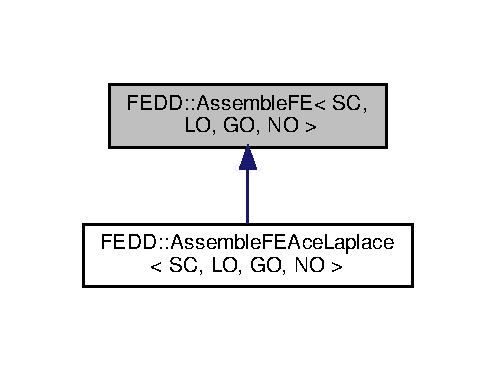
\includegraphics[width=350pt]{classFEDD_1_1AssembleFE__inherit__graph}
\end{center}
\end{figure}
\subsection*{Public Types}
\begin{DoxyCompactItemize}
\item 
typedef Small\+Matrix$<$ \hyperlink{fe__test__laplace_8cpp_a79c7e86a57edbb2a5a53242bcd04e41e}{SC} $>$ \hyperlink{classFEDD_1_1AssembleFE_a8b8c588ba0cfaa200a74215f19e62722}{Small\+Matrix\+\_\+\+Type}
\item 
typedef Teuchos\+::\+R\+CP$<$ \hyperlink{classFEDD_1_1AssembleFE_a8b8c588ba0cfaa200a74215f19e62722}{Small\+Matrix\+\_\+\+Type} $>$ \hyperlink{classFEDD_1_1AssembleFE_afb5fb5dca3aab59f697a25884e99e894}{Small\+Matrix\+Ptr\+\_\+\+Type}
\item 
typedef \hyperlink{classFEDD_1_1AssembleFE}{Assemble\+FE}$<$ \hyperlink{fe__test__laplace_8cpp_a79c7e86a57edbb2a5a53242bcd04e41e}{SC}, \hyperlink{fe__test__laplace_8cpp_ad6a38c9f07d3fd633eefca5bccad8410}{LO}, \hyperlink{fe__test__laplace_8cpp_afa2946b509009b4f45eb04bd8c5b27d9}{GO}, \hyperlink{fe__test__laplace_8cpp_a5e24f37b28787429872b6ecb1d0417ce}{NO} $>$ \hyperlink{classFEDD_1_1AssembleFE_ab2c8bb1fd65dfcf7899a7c4a4a8a4021}{Assemble\+F\+E\+\_\+\+Type}
\end{DoxyCompactItemize}
\subsection*{Public Member Functions}
\begin{DoxyCompactItemize}
\item 
virtual void \hyperlink{classFEDD_1_1AssembleFE_af48b450dfdf6cea7beeb24feef7dc10f}{assemble\+Jacobian} ()=0
\begin{DoxyCompactList}\small\item\em Assemble the element Jacobian matrix. \end{DoxyCompactList}\item 
virtual void \hyperlink{classFEDD_1_1AssembleFE_a43f18446faadb45bb4e2eae4f82ba9ba}{assemble\+R\+HS} ()=0
\begin{DoxyCompactList}\small\item\em Assemble the element right hand side vector. \end{DoxyCompactList}\item 
\hyperlink{classFEDD_1_1AssembleFE_afb5fb5dca3aab59f697a25884e99e894}{Small\+Matrix\+Ptr\+\_\+\+Type} \hyperlink{classFEDD_1_1AssembleFE_af7fb8c5ae1f77eca6e8c7e887ea761ec}{get\+Jacobian} ()
\begin{DoxyCompactList}\small\item\em Get the currently assembled element Jacobian matrix. \end{DoxyCompactList}\item 
vec\+\_\+dbl\+\_\+\+Type \hyperlink{classFEDD_1_1AssembleFE_a15f6f643268ff4571437bbb98b7325c5}{get\+R\+HS} ()
\begin{DoxyCompactList}\small\item\em Get the currently assembled right hand side vector. \end{DoxyCompactList}\item 
virtual void \hyperlink{classFEDD_1_1AssembleFE_a9d471f89532703a619e8a1545cab4602}{check\+Parameters} ()
\begin{DoxyCompactList}\small\item\em Check the input parameters from the constructor and the Parameter\+List for completeness and consistency. \end{DoxyCompactList}\item 
virtual void \hyperlink{classFEDD_1_1AssembleFE_a48ea6d9259f538a88fa5b21667869bce}{update\+Params} (Parameter\+List\+Ptr\+\_\+\+Type params)
\begin{DoxyCompactList}\small\item\em Set or update the parameters read from the Parameter\+List. \end{DoxyCompactList}\item 
void \hyperlink{classFEDD_1_1AssembleFE_aa291b30d2a3f78705b2a7722a1a04d96}{advance\+In\+Time} (double dt)
\begin{DoxyCompactList}\small\item\em This function is called every time the F\+E\+D\+D\+Lib proceeds from one to the next time step. The size of the time step will always be provided as input. \end{DoxyCompactList}\item 
double \hyperlink{classFEDD_1_1AssembleFE_a960875e7038a3f20e4507bc86f17247f}{get\+Time\+Step} ()
\begin{DoxyCompactList}\small\item\em Get the time state of the object. \end{DoxyCompactList}\item 
void \hyperlink{classFEDD_1_1AssembleFE_afbb44e574eb47e8e97436e9125f373a0}{advance\+Newton\+Step} ()
\begin{DoxyCompactList}\small\item\em This function is called every time the F\+E\+D\+D\+Lib proceeds from one to the next newton step. The size of the time step will always be provided as input. \end{DoxyCompactList}\item 
int \hyperlink{classFEDD_1_1AssembleFE_af11bbb371048522d35ecb1f4f2584a8a}{get\+Newton\+Step} ()
\begin{DoxyCompactList}\small\item\em Get the time state of the object. \end{DoxyCompactList}\item 
void \hyperlink{classFEDD_1_1AssembleFE_a5303adf0752fe27d9ff47ae8a39c1da4}{update\+Solution} (vec\+\_\+dbl\+\_\+\+Type solution)
\begin{DoxyCompactList}\small\item\em Update the solution vector. \end{DoxyCompactList}\item 
vec\+\_\+dbl\+\_\+\+Type \hyperlink{classFEDD_1_1AssembleFE_a33e83a1eb6656a74609dfbfaf3fae474}{get\+Solution} ()
\begin{DoxyCompactList}\small\item\em Get the current local solution vector. \end{DoxyCompactList}\item 
void \hyperlink{classFEDD_1_1AssembleFE_a7bfb3f6b49f102b0856551d62c8c8a9f}{pre\+Processing} ()
\begin{DoxyCompactList}\small\item\em This function is called in the beginning of each Newton step before actually assmblying anything. \end{DoxyCompactList}\item 
void \hyperlink{classFEDD_1_1AssembleFE_a8ae32f71020082d81b055afbeda6fc29}{post\+Processing} ()
\begin{DoxyCompactList}\small\item\em This function is called at the end of each Newton step after updating the solution vector. \end{DoxyCompactList}\item 
int \hyperlink{classFEDD_1_1AssembleFE_a35ada89164c74b433340733c01f30f4b}{get\+Dim} ()
\begin{DoxyCompactList}\small\item\em Get the spatial dimension. (Typically 2 or 3) \end{DoxyCompactList}\item 
vec2\+D\+\_\+dbl\+\_\+\+Type \hyperlink{classFEDD_1_1AssembleFE_a93f37b5e5f8f9a73152abb2e8be4ba4f}{get\+Nodes\+Ref\+Config} ()
\begin{DoxyCompactList}\small\item\em Return the coordnates of the finite element nodes. \end{DoxyCompactList}\item 
void \hyperlink{classFEDD_1_1AssembleFE_a9eea5124c4b385c2807ad8b20614d050}{add\+R\+H\+S\+Func} (Rhs\+Func\+\_\+\+Type rhs\+Func)
\item 
tuple\+\_\+sd\+\_\+vec\+\_\+ptr\+\_\+\+Type \hyperlink{classFEDD_1_1AssembleFE_a4d5d128fbd72747e01af917b16cee6f6}{get\+Tuple\+Element} ()
\begin{DoxyCompactList}\small\item\em Return tuple with element based values. first column per tuple string with description, second column value. \end{DoxyCompactList}\end{DoxyCompactItemize}
\subsection*{Protected Member Functions}
\begin{DoxyCompactItemize}
\item 
\hyperlink{classFEDD_1_1AssembleFE_a5ff56b610942ec92cc1b1e0ac1e07ce4}{Assemble\+FE} (int flag, vec2\+D\+\_\+dbl\+\_\+\+Type nodes\+Ref\+Config, Parameter\+List\+Ptr\+\_\+\+Type parameters, tuple\+\_\+disk\+\_\+vec\+\_\+ptr\+\_\+\+Type tuple)
\begin{DoxyCompactList}\small\item\em Constructor. \end{DoxyCompactList}\end{DoxyCompactItemize}
\subsection*{Protected Attributes}
\begin{DoxyCompactItemize}
\item 
\hyperlink{classFEDD_1_1AssembleFE_afb5fb5dca3aab59f697a25884e99e894}{Small\+Matrix\+Ptr\+\_\+\+Type} \hyperlink{classFEDD_1_1AssembleFE_a12d587892b238ecf6b8fdb0b91c2b0be}{jacobian\+\_\+}
\item 
vec\+\_\+dbl\+\_\+\+Type \hyperlink{classFEDD_1_1AssembleFE_a8eff2b1a9fc0125931206e83e2ab8bbd}{rhs\+Vec\+\_\+}
\item 
Rhs\+Func\+\_\+\+Type \hyperlink{classFEDD_1_1AssembleFE_a2c3232bc8b6d6d9e23ab0a745e103e2a}{rhs\+Func\+\_\+}
\item 
int \hyperlink{classFEDD_1_1AssembleFE_a8419f1d876b0da5f920ab3d1d21e0401}{dim\+\_\+}
\item 
tuple\+\_\+disk\+\_\+vec\+\_\+ptr\+\_\+\+Type \hyperlink{classFEDD_1_1AssembleFE_afd156e8e0ad2ca015a604290919d5794}{disk\+Tuple\+\_\+}
\item 
vec2\+D\+\_\+dbl\+\_\+\+Type \hyperlink{classFEDD_1_1AssembleFE_ab2892bff598d5a4f784d4f30ddf4836c}{nodes\+Ref\+Config\+\_\+}
\item 
bool \hyperlink{classFEDD_1_1AssembleFE_aaa84c5ca06ca8dcd1ad82d7d66ac8e4c}{time\+Problem\+\_\+}
\item 
int \hyperlink{classFEDD_1_1AssembleFE_a222f91cd1b4296d37a520e510692ca8e}{flag\+\_\+}
\item 
double \hyperlink{classFEDD_1_1AssembleFE_aedef52d32fc32f3b70877f705968afcc}{time\+Step\+\_\+}
\item 
int \hyperlink{classFEDD_1_1AssembleFE_a39520c726ee8a6a48258adc555f6df77}{newton\+Step\+\_\+}
\item 
Parameter\+List\+Ptr\+\_\+\+Type \hyperlink{classFEDD_1_1AssembleFE_ac270e80971846b789e7cb2507fe345ba}{params\+Material\+\_\+}
\item 
Parameter\+List\+Ptr\+\_\+\+Type \hyperlink{classFEDD_1_1AssembleFE_a1b7f9f820f3da30ff7dd8438ada14b3b}{params\+\_\+}
\item 
vec\+\_\+dbl\+\_\+\+Type \hyperlink{classFEDD_1_1AssembleFE_a5a0789e00592c0885abac42748c96fd7}{solution\+\_\+}
\end{DoxyCompactItemize}
\subsection*{Friends}
\begin{DoxyCompactItemize}
\item 
class \hyperlink{classFEDD_1_1AssembleFE_a30ff0dcd1d500892033fc319deacb8fb}{Assemble\+F\+E\+Factory$<$ S\+C, L\+O, G\+O, N\+O $>$}
\end{DoxyCompactItemize}


\subsection{Detailed Description}
\subsubsection*{template$<$class SC = default\+\_\+sc, class LO = default\+\_\+lo, class GO = default\+\_\+go, class NO = default\+\_\+no$>$\newline
class F\+E\+D\+D\+::\+Assemble\+F\+E$<$ S\+C, L\+O, G\+O, N\+O $>$}

This abstract class defining the interface for any type of element assembly rountines in the F\+E\+D\+D\+Lib. 


\begin{DoxyTemplParams}{Template Parameters}
{\em SC} & The scalar type. So far, this is always double, but having it as a template parameter would allow flexibily, e.\+g., for using complex instead \\
\hline
{\em LO} & The local ordinal type. The is the index type for local indices \\
\hline
{\em GO} & The global ordinal type. The is the index type for global indices \\
\hline
\end{DoxyTemplParams}
\begin{DoxyRefDesc}{Todo}
\item[\hyperlink{todo__todo000001}{Todo}]This should actually be removed since the class should operate only on element level) \end{DoxyRefDesc}

\begin{DoxyTemplParams}{Template Parameters}
{\em NO} & The Kokkos Node type. This would allow for performance portibility when using Kokkos. Currently, this is not used.\\
\hline
\end{DoxyTemplParams}
Any new assembly routine on element level should implemented following the interface provided in this class. During the setup of a specific boundary value problem one \hyperlink{classFEDD_1_1AssembleFE}{Assemble\+FE} object will be constructed using the \hyperlink{classFEDD_1_1AssembleFEFactory}{Assemble\+F\+E\+Factory} for each finite element. This is can be understood roughly as follows\+: 
\begin{DoxyCode}
\textcolor{keywordflow}{for} (\textcolor{keywordtype}{int} i=1; i<numElements; i++) \{
    \hyperlink{classFEDD_1_1AssembleFE_a5ff56b610942ec92cc1b1e0ac1e07ce4}{AssembleFE} assmeblyFe[i] = \hyperlink{classFEDD_1_1AssembleFEFactory_ac895d65acf2626100832586df84d6a9c}{AssembleFEFactory<>::build}(\textcolor{stringliteral}{"problemType"}
      ,flag,nodesRefConfig,params,tuple);
\}
\end{DoxyCode}
 It is not possible to construct an \hyperlink{classFEDD_1_1AssembleFE}{Assemble\+FE} object without using the \hyperlink{classFEDD_1_1AssembleFEFactory}{Assemble\+F\+E\+Factory} since the constructor is protected and hence not directly accessible.

Similar to constructing the \hyperlink{classFEDD_1_1AssembleFE}{Assemble\+FE}, all other member functions will be called automatically by the F\+E\+D\+D\+Lib during the program flow. For instance, the assembly of the element Jacobian matrices will be performed\+: 
\begin{DoxyCode}
\textcolor{keywordflow}{for} (\textcolor{keywordtype}{int} i=1; i<numElements; i++) \{
    assmeblyFe[i].assembleJacobian();
    Matrix\_Type elementJacobian[i] = assmeblyFe[i].getJacobian();
\}
\end{DoxyCode}
 A specific implementation of a class derived from \hyperlink{classFEDD_1_1AssembleFE}{Assemble\+FE} can only interact with the F\+E\+D\+D\+Lib by implementing the public member functions in \hyperlink{classFEDD_1_1AssembleFE}{Assemble\+FE} for
\begin{DoxyItemize}
\item Construction
\item Assmebly of the Jacobian and right hand side
\item Getting the Jacobian and right hand side
\item Upating the solution
\item ...
\end{DoxyItemize}

They will be automatically executed as the construction and assembly of the Jacobian; see above.

If additional public member functions are added, they will not be executed from the F\+E\+D\+D\+Lib. Therefore, we only allow for adding additional protected or private functions.

Upon construction, the F\+E\+D\+D\+Lib will provide some information, such as
\begin{DoxyItemize}
\item The element flag
\item The coordinates of the finite element nodes
\item ...
\end{DoxyItemize}

Additional parameters, such as material parameters, can provided through a Teuchos\+::\+Parameter\+List object which will contain all the parameters specified in the input file {\ttfamily A\+B\+C.\+xml}. The structure of the input file and, hence, of the resulting parameter list can be chosen freely depending on the specific implementation of an element assembly. The F\+E\+D\+D\+Lib will take care of reading the parameters from the file and making them available to every \hyperlink{classFEDD_1_1AssembleFE}{Assemble\+FE} object. 

\subsection{Member Typedef Documentation}
\mbox{\Hypertarget{classFEDD_1_1AssembleFE_ab2c8bb1fd65dfcf7899a7c4a4a8a4021}\label{classFEDD_1_1AssembleFE_ab2c8bb1fd65dfcf7899a7c4a4a8a4021}} 
\index{F\+E\+D\+D\+::\+Assemble\+FE@{F\+E\+D\+D\+::\+Assemble\+FE}!Assemble\+F\+E\+\_\+\+Type@{Assemble\+F\+E\+\_\+\+Type}}
\index{Assemble\+F\+E\+\_\+\+Type@{Assemble\+F\+E\+\_\+\+Type}!F\+E\+D\+D\+::\+Assemble\+FE@{F\+E\+D\+D\+::\+Assemble\+FE}}
\subsubsection{\texorpdfstring{Assemble\+F\+E\+\_\+\+Type}{AssembleFE\_Type}}
{\footnotesize\ttfamily template$<$class SC  = default\+\_\+sc, class LO  = default\+\_\+lo, class GO  = default\+\_\+go, class NO  = default\+\_\+no$>$ \\
typedef \hyperlink{classFEDD_1_1AssembleFE}{Assemble\+FE}$<$\hyperlink{fe__test__laplace_8cpp_a79c7e86a57edbb2a5a53242bcd04e41e}{SC},\hyperlink{fe__test__laplace_8cpp_ad6a38c9f07d3fd633eefca5bccad8410}{LO},\hyperlink{fe__test__laplace_8cpp_afa2946b509009b4f45eb04bd8c5b27d9}{GO},\hyperlink{fe__test__laplace_8cpp_a5e24f37b28787429872b6ecb1d0417ce}{NO}$>$ \hyperlink{classFEDD_1_1AssembleFE}{F\+E\+D\+D\+::\+Assemble\+FE}$<$ \hyperlink{fe__test__laplace_8cpp_a79c7e86a57edbb2a5a53242bcd04e41e}{SC}, \hyperlink{fe__test__laplace_8cpp_ad6a38c9f07d3fd633eefca5bccad8410}{LO}, \hyperlink{fe__test__laplace_8cpp_afa2946b509009b4f45eb04bd8c5b27d9}{GO}, \hyperlink{fe__test__laplace_8cpp_a5e24f37b28787429872b6ecb1d0417ce}{NO} $>$\+::\hyperlink{classFEDD_1_1AssembleFE_ab2c8bb1fd65dfcf7899a7c4a4a8a4021}{Assemble\+F\+E\+\_\+\+Type}}

\mbox{\Hypertarget{classFEDD_1_1AssembleFE_a8b8c588ba0cfaa200a74215f19e62722}\label{classFEDD_1_1AssembleFE_a8b8c588ba0cfaa200a74215f19e62722}} 
\index{F\+E\+D\+D\+::\+Assemble\+FE@{F\+E\+D\+D\+::\+Assemble\+FE}!Small\+Matrix\+\_\+\+Type@{Small\+Matrix\+\_\+\+Type}}
\index{Small\+Matrix\+\_\+\+Type@{Small\+Matrix\+\_\+\+Type}!F\+E\+D\+D\+::\+Assemble\+FE@{F\+E\+D\+D\+::\+Assemble\+FE}}
\subsubsection{\texorpdfstring{Small\+Matrix\+\_\+\+Type}{SmallMatrix\_Type}}
{\footnotesize\ttfamily template$<$class SC  = default\+\_\+sc, class LO  = default\+\_\+lo, class GO  = default\+\_\+go, class NO  = default\+\_\+no$>$ \\
typedef Small\+Matrix$<$\hyperlink{fe__test__laplace_8cpp_a79c7e86a57edbb2a5a53242bcd04e41e}{SC}$>$ \hyperlink{classFEDD_1_1AssembleFE}{F\+E\+D\+D\+::\+Assemble\+FE}$<$ \hyperlink{fe__test__laplace_8cpp_a79c7e86a57edbb2a5a53242bcd04e41e}{SC}, \hyperlink{fe__test__laplace_8cpp_ad6a38c9f07d3fd633eefca5bccad8410}{LO}, \hyperlink{fe__test__laplace_8cpp_afa2946b509009b4f45eb04bd8c5b27d9}{GO}, \hyperlink{fe__test__laplace_8cpp_a5e24f37b28787429872b6ecb1d0417ce}{NO} $>$\+::\hyperlink{classFEDD_1_1AssembleFE_a8b8c588ba0cfaa200a74215f19e62722}{Small\+Matrix\+\_\+\+Type}}

\mbox{\Hypertarget{classFEDD_1_1AssembleFE_afb5fb5dca3aab59f697a25884e99e894}\label{classFEDD_1_1AssembleFE_afb5fb5dca3aab59f697a25884e99e894}} 
\index{F\+E\+D\+D\+::\+Assemble\+FE@{F\+E\+D\+D\+::\+Assemble\+FE}!Small\+Matrix\+Ptr\+\_\+\+Type@{Small\+Matrix\+Ptr\+\_\+\+Type}}
\index{Small\+Matrix\+Ptr\+\_\+\+Type@{Small\+Matrix\+Ptr\+\_\+\+Type}!F\+E\+D\+D\+::\+Assemble\+FE@{F\+E\+D\+D\+::\+Assemble\+FE}}
\subsubsection{\texorpdfstring{Small\+Matrix\+Ptr\+\_\+\+Type}{SmallMatrixPtr\_Type}}
{\footnotesize\ttfamily template$<$class SC  = default\+\_\+sc, class LO  = default\+\_\+lo, class GO  = default\+\_\+go, class NO  = default\+\_\+no$>$ \\
typedef Teuchos\+::\+R\+CP$<$\hyperlink{classFEDD_1_1AssembleFE_a8b8c588ba0cfaa200a74215f19e62722}{Small\+Matrix\+\_\+\+Type}$>$ \hyperlink{classFEDD_1_1AssembleFE}{F\+E\+D\+D\+::\+Assemble\+FE}$<$ \hyperlink{fe__test__laplace_8cpp_a79c7e86a57edbb2a5a53242bcd04e41e}{SC}, \hyperlink{fe__test__laplace_8cpp_ad6a38c9f07d3fd633eefca5bccad8410}{LO}, \hyperlink{fe__test__laplace_8cpp_afa2946b509009b4f45eb04bd8c5b27d9}{GO}, \hyperlink{fe__test__laplace_8cpp_a5e24f37b28787429872b6ecb1d0417ce}{NO} $>$\+::\hyperlink{classFEDD_1_1AssembleFE_afb5fb5dca3aab59f697a25884e99e894}{Small\+Matrix\+Ptr\+\_\+\+Type}}



\subsection{Constructor \& Destructor Documentation}
\mbox{\Hypertarget{classFEDD_1_1AssembleFE_a5ff56b610942ec92cc1b1e0ac1e07ce4}\label{classFEDD_1_1AssembleFE_a5ff56b610942ec92cc1b1e0ac1e07ce4}} 
\index{F\+E\+D\+D\+::\+Assemble\+FE@{F\+E\+D\+D\+::\+Assemble\+FE}!Assemble\+FE@{Assemble\+FE}}
\index{Assemble\+FE@{Assemble\+FE}!F\+E\+D\+D\+::\+Assemble\+FE@{F\+E\+D\+D\+::\+Assemble\+FE}}
\subsubsection{\texorpdfstring{Assemble\+F\+E()}{AssembleFE()}}
{\footnotesize\ttfamily template$<$class SC , class LO , class GO , class NO $>$ \\
\hyperlink{classFEDD_1_1AssembleFE}{F\+E\+D\+D\+::\+Assemble\+FE}$<$ \hyperlink{fe__test__laplace_8cpp_a79c7e86a57edbb2a5a53242bcd04e41e}{SC}, \hyperlink{fe__test__laplace_8cpp_ad6a38c9f07d3fd633eefca5bccad8410}{LO}, \hyperlink{fe__test__laplace_8cpp_afa2946b509009b4f45eb04bd8c5b27d9}{GO}, \hyperlink{fe__test__laplace_8cpp_a5e24f37b28787429872b6ecb1d0417ce}{NO} $>$\+::\hyperlink{classFEDD_1_1AssembleFE}{Assemble\+FE} (\begin{DoxyParamCaption}\item[{int}]{flag,  }\item[{vec2\+D\+\_\+dbl\+\_\+\+Type}]{nodes\+Ref\+Config,  }\item[{Parameter\+List\+Ptr\+\_\+\+Type}]{parameters,  }\item[{tuple\+\_\+disk\+\_\+vec\+\_\+ptr\+\_\+\+Type}]{tuple }\end{DoxyParamCaption})\hspace{0.3cm}{\ttfamily [protected]}}



Constructor. 


\begin{DoxyParams}[1]{Parameters}
\mbox{\tt in}  & {\em flag} & Flag of element \\
\hline
\mbox{\tt in}  & {\em nodes\+Ref\+Config} & Nodes of element in reference configuration \\
\hline
\mbox{\tt in}  & {\em params} & Parameterlist for current problem \\
\hline
\mbox{\tt in}  & {\em tuple} & vector of element information tuples. \\
\hline
\end{DoxyParams}
Element Numbering for triangular elements\+:

\begin{DoxyVerb}- Triangle numbering

                2
                *
                *
          4     5
                *
                *
    1 * * 3 * * 0
\end{DoxyVerb}
 



\begin{DoxyVerb}- Tetrahedral numbering

            Face 1          Face2               Face 3            Face 4
                2      2 * * 9 * * 3        3 * * 9 * * 2            3
                *      *          *          *          *           * *
                *      *        *             *        *          *   *
          5     6      6      7                8      5         8     7
                *      *    *                   *    *        *       *
                *      *  *                      *  *       *         *
    1 * * 4 * * 0       0                         1       1 * * 4 * * 0
\end{DoxyVerb}
 



\subsection{Member Function Documentation}
\mbox{\Hypertarget{classFEDD_1_1AssembleFE_a9eea5124c4b385c2807ad8b20614d050}\label{classFEDD_1_1AssembleFE_a9eea5124c4b385c2807ad8b20614d050}} 
\index{F\+E\+D\+D\+::\+Assemble\+FE@{F\+E\+D\+D\+::\+Assemble\+FE}!add\+R\+H\+S\+Func@{add\+R\+H\+S\+Func}}
\index{add\+R\+H\+S\+Func@{add\+R\+H\+S\+Func}!F\+E\+D\+D\+::\+Assemble\+FE@{F\+E\+D\+D\+::\+Assemble\+FE}}
\subsubsection{\texorpdfstring{add\+R\+H\+S\+Func()}{addRHSFunc()}}
{\footnotesize\ttfamily template$<$class SC  = default\+\_\+sc, class LO  = default\+\_\+lo, class GO  = default\+\_\+go, class NO  = default\+\_\+no$>$ \\
void \hyperlink{classFEDD_1_1AssembleFE}{F\+E\+D\+D\+::\+Assemble\+FE}$<$ \hyperlink{fe__test__laplace_8cpp_a79c7e86a57edbb2a5a53242bcd04e41e}{SC}, \hyperlink{fe__test__laplace_8cpp_ad6a38c9f07d3fd633eefca5bccad8410}{LO}, \hyperlink{fe__test__laplace_8cpp_afa2946b509009b4f45eb04bd8c5b27d9}{GO}, \hyperlink{fe__test__laplace_8cpp_a5e24f37b28787429872b6ecb1d0417ce}{NO} $>$\+::add\+R\+H\+S\+Func (\begin{DoxyParamCaption}\item[{Rhs\+Func\+\_\+\+Type}]{rhs\+Func }\end{DoxyParamCaption})\hspace{0.3cm}{\ttfamily [inline]}}

\begin{DoxyRefDesc}{Todo}
\item[\hyperlink{todo__todo000005}{Todo}]Still work in Progress with R\+HS and Mass Matrix \end{DoxyRefDesc}
\mbox{\Hypertarget{classFEDD_1_1AssembleFE_aa291b30d2a3f78705b2a7722a1a04d96}\label{classFEDD_1_1AssembleFE_aa291b30d2a3f78705b2a7722a1a04d96}} 
\index{F\+E\+D\+D\+::\+Assemble\+FE@{F\+E\+D\+D\+::\+Assemble\+FE}!advance\+In\+Time@{advance\+In\+Time}}
\index{advance\+In\+Time@{advance\+In\+Time}!F\+E\+D\+D\+::\+Assemble\+FE@{F\+E\+D\+D\+::\+Assemble\+FE}}
\subsubsection{\texorpdfstring{advance\+In\+Time()}{advanceInTime()}}
{\footnotesize\ttfamily template$<$class SC , class LO , class GO , class NO $>$ \\
void \hyperlink{classFEDD_1_1AssembleFE}{F\+E\+D\+D\+::\+Assemble\+FE}$<$ \hyperlink{fe__test__laplace_8cpp_a79c7e86a57edbb2a5a53242bcd04e41e}{SC}, \hyperlink{fe__test__laplace_8cpp_ad6a38c9f07d3fd633eefca5bccad8410}{LO}, \hyperlink{fe__test__laplace_8cpp_afa2946b509009b4f45eb04bd8c5b27d9}{GO}, \hyperlink{fe__test__laplace_8cpp_a5e24f37b28787429872b6ecb1d0417ce}{NO} $>$\+::advance\+In\+Time (\begin{DoxyParamCaption}\item[{double}]{dt }\end{DoxyParamCaption})}



This function is called every time the F\+E\+D\+D\+Lib proceeds from one to the next time step. The size of the time step will always be provided as input. 


\begin{DoxyParams}[1]{Parameters}
\mbox{\tt in}  & {\em dt} & Timestepping length \\
\hline
\end{DoxyParams}
\mbox{\Hypertarget{classFEDD_1_1AssembleFE_afbb44e574eb47e8e97436e9125f373a0}\label{classFEDD_1_1AssembleFE_afbb44e574eb47e8e97436e9125f373a0}} 
\index{F\+E\+D\+D\+::\+Assemble\+FE@{F\+E\+D\+D\+::\+Assemble\+FE}!advance\+Newton\+Step@{advance\+Newton\+Step}}
\index{advance\+Newton\+Step@{advance\+Newton\+Step}!F\+E\+D\+D\+::\+Assemble\+FE@{F\+E\+D\+D\+::\+Assemble\+FE}}
\subsubsection{\texorpdfstring{advance\+Newton\+Step()}{advanceNewtonStep()}}
{\footnotesize\ttfamily template$<$class SC , class LO , class GO , class NO $>$ \\
void \hyperlink{classFEDD_1_1AssembleFE}{F\+E\+D\+D\+::\+Assemble\+FE}$<$ \hyperlink{fe__test__laplace_8cpp_a79c7e86a57edbb2a5a53242bcd04e41e}{SC}, \hyperlink{fe__test__laplace_8cpp_ad6a38c9f07d3fd633eefca5bccad8410}{LO}, \hyperlink{fe__test__laplace_8cpp_afa2946b509009b4f45eb04bd8c5b27d9}{GO}, \hyperlink{fe__test__laplace_8cpp_a5e24f37b28787429872b6ecb1d0417ce}{NO} $>$\+::advance\+Newton\+Step (\begin{DoxyParamCaption}{ }\end{DoxyParamCaption})}



This function is called every time the F\+E\+D\+D\+Lib proceeds from one to the next newton step. The size of the time step will always be provided as input. 

\mbox{\Hypertarget{classFEDD_1_1AssembleFE_af48b450dfdf6cea7beeb24feef7dc10f}\label{classFEDD_1_1AssembleFE_af48b450dfdf6cea7beeb24feef7dc10f}} 
\index{F\+E\+D\+D\+::\+Assemble\+FE@{F\+E\+D\+D\+::\+Assemble\+FE}!assemble\+Jacobian@{assemble\+Jacobian}}
\index{assemble\+Jacobian@{assemble\+Jacobian}!F\+E\+D\+D\+::\+Assemble\+FE@{F\+E\+D\+D\+::\+Assemble\+FE}}
\subsubsection{\texorpdfstring{assemble\+Jacobian()}{assembleJacobian()}}
{\footnotesize\ttfamily template$<$class SC  = default\+\_\+sc, class LO  = default\+\_\+lo, class GO  = default\+\_\+go, class NO  = default\+\_\+no$>$ \\
virtual void \hyperlink{classFEDD_1_1AssembleFE}{F\+E\+D\+D\+::\+Assemble\+FE}$<$ \hyperlink{fe__test__laplace_8cpp_a79c7e86a57edbb2a5a53242bcd04e41e}{SC}, \hyperlink{fe__test__laplace_8cpp_ad6a38c9f07d3fd633eefca5bccad8410}{LO}, \hyperlink{fe__test__laplace_8cpp_afa2946b509009b4f45eb04bd8c5b27d9}{GO}, \hyperlink{fe__test__laplace_8cpp_a5e24f37b28787429872b6ecb1d0417ce}{NO} $>$\+::assemble\+Jacobian (\begin{DoxyParamCaption}{ }\end{DoxyParamCaption})\hspace{0.3cm}{\ttfamily [pure virtual]}}



Assemble the element Jacobian matrix. 

\begin{DoxyReturn}{Returns}
the element Jacobian matrix 
\end{DoxyReturn}


Implemented in \hyperlink{classFEDD_1_1AssembleFEAceLaplace_ac47ac062ba522289f4e9a5dd2df78503}{F\+E\+D\+D\+::\+Assemble\+F\+E\+Ace\+Laplace$<$ S\+C, L\+O, G\+O, N\+O $>$}, and \hyperlink{classFEDD_1_1AssembleFEAceNavierStokes_a1535786ac6b897da287e3e7e0aa60f61}{F\+E\+D\+D\+::\+Assemble\+F\+E\+Ace\+Navier\+Stokes$<$ S\+C, L\+O, G\+O, N\+O $>$}.

\mbox{\Hypertarget{classFEDD_1_1AssembleFE_a43f18446faadb45bb4e2eae4f82ba9ba}\label{classFEDD_1_1AssembleFE_a43f18446faadb45bb4e2eae4f82ba9ba}} 
\index{F\+E\+D\+D\+::\+Assemble\+FE@{F\+E\+D\+D\+::\+Assemble\+FE}!assemble\+R\+HS@{assemble\+R\+HS}}
\index{assemble\+R\+HS@{assemble\+R\+HS}!F\+E\+D\+D\+::\+Assemble\+FE@{F\+E\+D\+D\+::\+Assemble\+FE}}
\subsubsection{\texorpdfstring{assemble\+R\+H\+S()}{assembleRHS()}}
{\footnotesize\ttfamily template$<$class SC  = default\+\_\+sc, class LO  = default\+\_\+lo, class GO  = default\+\_\+go, class NO  = default\+\_\+no$>$ \\
virtual void \hyperlink{classFEDD_1_1AssembleFE}{F\+E\+D\+D\+::\+Assemble\+FE}$<$ \hyperlink{fe__test__laplace_8cpp_a79c7e86a57edbb2a5a53242bcd04e41e}{SC}, \hyperlink{fe__test__laplace_8cpp_ad6a38c9f07d3fd633eefca5bccad8410}{LO}, \hyperlink{fe__test__laplace_8cpp_afa2946b509009b4f45eb04bd8c5b27d9}{GO}, \hyperlink{fe__test__laplace_8cpp_a5e24f37b28787429872b6ecb1d0417ce}{NO} $>$\+::assemble\+R\+HS (\begin{DoxyParamCaption}{ }\end{DoxyParamCaption})\hspace{0.3cm}{\ttfamily [pure virtual]}}



Assemble the element right hand side vector. 

\begin{DoxyReturn}{Returns}
the element right hand side vector 
\end{DoxyReturn}


Implemented in \hyperlink{classFEDD_1_1AssembleFEAceLaplace_a6d2759738ff7b596b4f132bf234c772a}{F\+E\+D\+D\+::\+Assemble\+F\+E\+Ace\+Laplace$<$ S\+C, L\+O, G\+O, N\+O $>$}, and \hyperlink{classFEDD_1_1AssembleFEAceNavierStokes_af42c6437fdac694ffbdccd12f8c581f2}{F\+E\+D\+D\+::\+Assemble\+F\+E\+Ace\+Navier\+Stokes$<$ S\+C, L\+O, G\+O, N\+O $>$}.

\mbox{\Hypertarget{classFEDD_1_1AssembleFE_a9d471f89532703a619e8a1545cab4602}\label{classFEDD_1_1AssembleFE_a9d471f89532703a619e8a1545cab4602}} 
\index{F\+E\+D\+D\+::\+Assemble\+FE@{F\+E\+D\+D\+::\+Assemble\+FE}!check\+Parameters@{check\+Parameters}}
\index{check\+Parameters@{check\+Parameters}!F\+E\+D\+D\+::\+Assemble\+FE@{F\+E\+D\+D\+::\+Assemble\+FE}}
\subsubsection{\texorpdfstring{check\+Parameters()}{checkParameters()}}
{\footnotesize\ttfamily template$<$class SC , class LO , class GO , class NO $>$ \\
void \hyperlink{classFEDD_1_1AssembleFE}{F\+E\+D\+D\+::\+Assemble\+FE}$<$ \hyperlink{fe__test__laplace_8cpp_a79c7e86a57edbb2a5a53242bcd04e41e}{SC}, \hyperlink{fe__test__laplace_8cpp_ad6a38c9f07d3fd633eefca5bccad8410}{LO}, \hyperlink{fe__test__laplace_8cpp_afa2946b509009b4f45eb04bd8c5b27d9}{GO}, \hyperlink{fe__test__laplace_8cpp_a5e24f37b28787429872b6ecb1d0417ce}{NO} $>$\+::check\+Parameters (\begin{DoxyParamCaption}{ }\end{DoxyParamCaption})\hspace{0.3cm}{\ttfamily [virtual]}}



Check the input parameters from the constructor and the Parameter\+List for completeness and consistency. 

\mbox{\Hypertarget{classFEDD_1_1AssembleFE_a35ada89164c74b433340733c01f30f4b}\label{classFEDD_1_1AssembleFE_a35ada89164c74b433340733c01f30f4b}} 
\index{F\+E\+D\+D\+::\+Assemble\+FE@{F\+E\+D\+D\+::\+Assemble\+FE}!get\+Dim@{get\+Dim}}
\index{get\+Dim@{get\+Dim}!F\+E\+D\+D\+::\+Assemble\+FE@{F\+E\+D\+D\+::\+Assemble\+FE}}
\subsubsection{\texorpdfstring{get\+Dim()}{getDim()}}
{\footnotesize\ttfamily template$<$class SC , class LO , class GO , class NO $>$ \\
int \hyperlink{classFEDD_1_1AssembleFE}{F\+E\+D\+D\+::\+Assemble\+FE}$<$ \hyperlink{fe__test__laplace_8cpp_a79c7e86a57edbb2a5a53242bcd04e41e}{SC}, \hyperlink{fe__test__laplace_8cpp_ad6a38c9f07d3fd633eefca5bccad8410}{LO}, \hyperlink{fe__test__laplace_8cpp_afa2946b509009b4f45eb04bd8c5b27d9}{GO}, \hyperlink{fe__test__laplace_8cpp_a5e24f37b28787429872b6ecb1d0417ce}{NO} $>$\+::get\+Dim (\begin{DoxyParamCaption}{ }\end{DoxyParamCaption})}



Get the spatial dimension. (Typically 2 or 3) 

\begin{DoxyRefDesc}{Todo}
\item[\hyperlink{todo__todo000003}{Todo}]Post\+Processing\+: Teuchos\+::\+Array with values and one global Array with Strings and names \end{DoxyRefDesc}


\begin{DoxyReturn}{Returns}
dimension. 
\end{DoxyReturn}
\mbox{\Hypertarget{classFEDD_1_1AssembleFE_af7fb8c5ae1f77eca6e8c7e887ea761ec}\label{classFEDD_1_1AssembleFE_af7fb8c5ae1f77eca6e8c7e887ea761ec}} 
\index{F\+E\+D\+D\+::\+Assemble\+FE@{F\+E\+D\+D\+::\+Assemble\+FE}!get\+Jacobian@{get\+Jacobian}}
\index{get\+Jacobian@{get\+Jacobian}!F\+E\+D\+D\+::\+Assemble\+FE@{F\+E\+D\+D\+::\+Assemble\+FE}}
\subsubsection{\texorpdfstring{get\+Jacobian()}{getJacobian()}}
{\footnotesize\ttfamily template$<$class SC  = default\+\_\+sc, class LO  = default\+\_\+lo, class GO  = default\+\_\+go, class NO  = default\+\_\+no$>$ \\
\hyperlink{classFEDD_1_1AssembleFE_afb5fb5dca3aab59f697a25884e99e894}{Small\+Matrix\+Ptr\+\_\+\+Type} \hyperlink{classFEDD_1_1AssembleFE}{F\+E\+D\+D\+::\+Assemble\+FE}$<$ \hyperlink{fe__test__laplace_8cpp_a79c7e86a57edbb2a5a53242bcd04e41e}{SC}, \hyperlink{fe__test__laplace_8cpp_ad6a38c9f07d3fd633eefca5bccad8410}{LO}, \hyperlink{fe__test__laplace_8cpp_afa2946b509009b4f45eb04bd8c5b27d9}{GO}, \hyperlink{fe__test__laplace_8cpp_a5e24f37b28787429872b6ecb1d0417ce}{NO} $>$\+::get\+Jacobian (\begin{DoxyParamCaption}{ }\end{DoxyParamCaption})\hspace{0.3cm}{\ttfamily [inline]}}



Get the currently assembled element Jacobian matrix. 

\begin{DoxyReturn}{Returns}
the element Jacobian matrix 
\end{DoxyReturn}
\mbox{\Hypertarget{classFEDD_1_1AssembleFE_af11bbb371048522d35ecb1f4f2584a8a}\label{classFEDD_1_1AssembleFE_af11bbb371048522d35ecb1f4f2584a8a}} 
\index{F\+E\+D\+D\+::\+Assemble\+FE@{F\+E\+D\+D\+::\+Assemble\+FE}!get\+Newton\+Step@{get\+Newton\+Step}}
\index{get\+Newton\+Step@{get\+Newton\+Step}!F\+E\+D\+D\+::\+Assemble\+FE@{F\+E\+D\+D\+::\+Assemble\+FE}}
\subsubsection{\texorpdfstring{get\+Newton\+Step()}{getNewtonStep()}}
{\footnotesize\ttfamily template$<$class SC , class LO , class GO , class NO $>$ \\
int \hyperlink{classFEDD_1_1AssembleFE}{F\+E\+D\+D\+::\+Assemble\+FE}$<$ \hyperlink{fe__test__laplace_8cpp_a79c7e86a57edbb2a5a53242bcd04e41e}{SC}, \hyperlink{fe__test__laplace_8cpp_ad6a38c9f07d3fd633eefca5bccad8410}{LO}, \hyperlink{fe__test__laplace_8cpp_afa2946b509009b4f45eb04bd8c5b27d9}{GO}, \hyperlink{fe__test__laplace_8cpp_a5e24f37b28787429872b6ecb1d0417ce}{NO} $>$\+::get\+Newton\+Step (\begin{DoxyParamCaption}{ }\end{DoxyParamCaption})}



Get the time state of the object. 

\begin{DoxyReturn}{Returns}
newton\+Step. 
\end{DoxyReturn}
\mbox{\Hypertarget{classFEDD_1_1AssembleFE_a93f37b5e5f8f9a73152abb2e8be4ba4f}\label{classFEDD_1_1AssembleFE_a93f37b5e5f8f9a73152abb2e8be4ba4f}} 
\index{F\+E\+D\+D\+::\+Assemble\+FE@{F\+E\+D\+D\+::\+Assemble\+FE}!get\+Nodes\+Ref\+Config@{get\+Nodes\+Ref\+Config}}
\index{get\+Nodes\+Ref\+Config@{get\+Nodes\+Ref\+Config}!F\+E\+D\+D\+::\+Assemble\+FE@{F\+E\+D\+D\+::\+Assemble\+FE}}
\subsubsection{\texorpdfstring{get\+Nodes\+Ref\+Config()}{getNodesRefConfig()}}
{\footnotesize\ttfamily template$<$class SC , class LO , class GO , class NO $>$ \\
vec2\+D\+\_\+dbl\+\_\+\+Type \hyperlink{classFEDD_1_1AssembleFE}{F\+E\+D\+D\+::\+Assemble\+FE}$<$ \hyperlink{fe__test__laplace_8cpp_a79c7e86a57edbb2a5a53242bcd04e41e}{SC}, \hyperlink{fe__test__laplace_8cpp_ad6a38c9f07d3fd633eefca5bccad8410}{LO}, \hyperlink{fe__test__laplace_8cpp_afa2946b509009b4f45eb04bd8c5b27d9}{GO}, \hyperlink{fe__test__laplace_8cpp_a5e24f37b28787429872b6ecb1d0417ce}{NO} $>$\+::get\+Nodes\+Ref\+Config (\begin{DoxyParamCaption}{ }\end{DoxyParamCaption})}



Return the coordnates of the finite element nodes. 

\begin{DoxyReturn}{Returns}
a 2D array with the coordnates for each nodes 
\end{DoxyReturn}
\begin{DoxyRefDesc}{Todo}
\item[\hyperlink{todo__todo000004}{Todo}]How is the ordering? \end{DoxyRefDesc}
\mbox{\Hypertarget{classFEDD_1_1AssembleFE_a15f6f643268ff4571437bbb98b7325c5}\label{classFEDD_1_1AssembleFE_a15f6f643268ff4571437bbb98b7325c5}} 
\index{F\+E\+D\+D\+::\+Assemble\+FE@{F\+E\+D\+D\+::\+Assemble\+FE}!get\+R\+HS@{get\+R\+HS}}
\index{get\+R\+HS@{get\+R\+HS}!F\+E\+D\+D\+::\+Assemble\+FE@{F\+E\+D\+D\+::\+Assemble\+FE}}
\subsubsection{\texorpdfstring{get\+R\+H\+S()}{getRHS()}}
{\footnotesize\ttfamily template$<$class SC  = default\+\_\+sc, class LO  = default\+\_\+lo, class GO  = default\+\_\+go, class NO  = default\+\_\+no$>$ \\
vec\+\_\+dbl\+\_\+\+Type \hyperlink{classFEDD_1_1AssembleFE}{F\+E\+D\+D\+::\+Assemble\+FE}$<$ \hyperlink{fe__test__laplace_8cpp_a79c7e86a57edbb2a5a53242bcd04e41e}{SC}, \hyperlink{fe__test__laplace_8cpp_ad6a38c9f07d3fd633eefca5bccad8410}{LO}, \hyperlink{fe__test__laplace_8cpp_afa2946b509009b4f45eb04bd8c5b27d9}{GO}, \hyperlink{fe__test__laplace_8cpp_a5e24f37b28787429872b6ecb1d0417ce}{NO} $>$\+::get\+R\+HS (\begin{DoxyParamCaption}{ }\end{DoxyParamCaption})\hspace{0.3cm}{\ttfamily [inline]}}



Get the currently assembled right hand side vector. 

\begin{DoxyReturn}{Returns}
the element right hand side vector 
\end{DoxyReturn}
\mbox{\Hypertarget{classFEDD_1_1AssembleFE_a33e83a1eb6656a74609dfbfaf3fae474}\label{classFEDD_1_1AssembleFE_a33e83a1eb6656a74609dfbfaf3fae474}} 
\index{F\+E\+D\+D\+::\+Assemble\+FE@{F\+E\+D\+D\+::\+Assemble\+FE}!get\+Solution@{get\+Solution}}
\index{get\+Solution@{get\+Solution}!F\+E\+D\+D\+::\+Assemble\+FE@{F\+E\+D\+D\+::\+Assemble\+FE}}
\subsubsection{\texorpdfstring{get\+Solution()}{getSolution()}}
{\footnotesize\ttfamily template$<$class SC , class LO , class GO , class NO $>$ \\
vec\+\_\+dbl\+\_\+\+Type \hyperlink{classFEDD_1_1AssembleFE}{F\+E\+D\+D\+::\+Assemble\+FE}$<$ \hyperlink{fe__test__laplace_8cpp_a79c7e86a57edbb2a5a53242bcd04e41e}{SC}, \hyperlink{fe__test__laplace_8cpp_ad6a38c9f07d3fd633eefca5bccad8410}{LO}, \hyperlink{fe__test__laplace_8cpp_afa2946b509009b4f45eb04bd8c5b27d9}{GO}, \hyperlink{fe__test__laplace_8cpp_a5e24f37b28787429872b6ecb1d0417ce}{NO} $>$\+::get\+Solution (\begin{DoxyParamCaption}{ }\end{DoxyParamCaption})}



Get the current local solution vector. 

\begin{DoxyReturn}{Returns}
the solution vector. 
\end{DoxyReturn}
\mbox{\Hypertarget{classFEDD_1_1AssembleFE_a960875e7038a3f20e4507bc86f17247f}\label{classFEDD_1_1AssembleFE_a960875e7038a3f20e4507bc86f17247f}} 
\index{F\+E\+D\+D\+::\+Assemble\+FE@{F\+E\+D\+D\+::\+Assemble\+FE}!get\+Time\+Step@{get\+Time\+Step}}
\index{get\+Time\+Step@{get\+Time\+Step}!F\+E\+D\+D\+::\+Assemble\+FE@{F\+E\+D\+D\+::\+Assemble\+FE}}
\subsubsection{\texorpdfstring{get\+Time\+Step()}{getTimeStep()}}
{\footnotesize\ttfamily template$<$class SC , class LO , class GO , class NO $>$ \\
double \hyperlink{classFEDD_1_1AssembleFE}{F\+E\+D\+D\+::\+Assemble\+FE}$<$ \hyperlink{fe__test__laplace_8cpp_a79c7e86a57edbb2a5a53242bcd04e41e}{SC}, \hyperlink{fe__test__laplace_8cpp_ad6a38c9f07d3fd633eefca5bccad8410}{LO}, \hyperlink{fe__test__laplace_8cpp_afa2946b509009b4f45eb04bd8c5b27d9}{GO}, \hyperlink{fe__test__laplace_8cpp_a5e24f37b28787429872b6ecb1d0417ce}{NO} $>$\+::get\+Time\+Step (\begin{DoxyParamCaption}{ }\end{DoxyParamCaption})}



Get the time state of the object. 

\begin{DoxyReturn}{Returns}
the timestep 
\end{DoxyReturn}
\mbox{\Hypertarget{classFEDD_1_1AssembleFE_a4d5d128fbd72747e01af917b16cee6f6}\label{classFEDD_1_1AssembleFE_a4d5d128fbd72747e01af917b16cee6f6}} 
\index{F\+E\+D\+D\+::\+Assemble\+FE@{F\+E\+D\+D\+::\+Assemble\+FE}!get\+Tuple\+Element@{get\+Tuple\+Element}}
\index{get\+Tuple\+Element@{get\+Tuple\+Element}!F\+E\+D\+D\+::\+Assemble\+FE@{F\+E\+D\+D\+::\+Assemble\+FE}}
\subsubsection{\texorpdfstring{get\+Tuple\+Element()}{getTupleElement()}}
{\footnotesize\ttfamily template$<$class SC  = default\+\_\+sc, class LO  = default\+\_\+lo, class GO  = default\+\_\+go, class NO  = default\+\_\+no$>$ \\
tuple\+\_\+sd\+\_\+vec\+\_\+ptr\+\_\+\+Type \hyperlink{classFEDD_1_1AssembleFE}{F\+E\+D\+D\+::\+Assemble\+FE}$<$ \hyperlink{fe__test__laplace_8cpp_a79c7e86a57edbb2a5a53242bcd04e41e}{SC}, \hyperlink{fe__test__laplace_8cpp_ad6a38c9f07d3fd633eefca5bccad8410}{LO}, \hyperlink{fe__test__laplace_8cpp_afa2946b509009b4f45eb04bd8c5b27d9}{GO}, \hyperlink{fe__test__laplace_8cpp_a5e24f37b28787429872b6ecb1d0417ce}{NO} $>$\+::get\+Tuple\+Element (\begin{DoxyParamCaption}{ }\end{DoxyParamCaption})}



Return tuple with element based values. first column per tuple string with description, second column value. 

\mbox{\Hypertarget{classFEDD_1_1AssembleFE_a8ae32f71020082d81b055afbeda6fc29}\label{classFEDD_1_1AssembleFE_a8ae32f71020082d81b055afbeda6fc29}} 
\index{F\+E\+D\+D\+::\+Assemble\+FE@{F\+E\+D\+D\+::\+Assemble\+FE}!post\+Processing@{post\+Processing}}
\index{post\+Processing@{post\+Processing}!F\+E\+D\+D\+::\+Assemble\+FE@{F\+E\+D\+D\+::\+Assemble\+FE}}
\subsubsection{\texorpdfstring{post\+Processing()}{postProcessing()}}
{\footnotesize\ttfamily template$<$class SC , class LO , class GO , class NO $>$ \\
void \hyperlink{classFEDD_1_1AssembleFE}{F\+E\+D\+D\+::\+Assemble\+FE}$<$ \hyperlink{fe__test__laplace_8cpp_a79c7e86a57edbb2a5a53242bcd04e41e}{SC}, \hyperlink{fe__test__laplace_8cpp_ad6a38c9f07d3fd633eefca5bccad8410}{LO}, \hyperlink{fe__test__laplace_8cpp_afa2946b509009b4f45eb04bd8c5b27d9}{GO}, \hyperlink{fe__test__laplace_8cpp_a5e24f37b28787429872b6ecb1d0417ce}{NO} $>$\+::post\+Processing (\begin{DoxyParamCaption}{ }\end{DoxyParamCaption})}



This function is called at the end of each Newton step after updating the solution vector. 

\mbox{\Hypertarget{classFEDD_1_1AssembleFE_a7bfb3f6b49f102b0856551d62c8c8a9f}\label{classFEDD_1_1AssembleFE_a7bfb3f6b49f102b0856551d62c8c8a9f}} 
\index{F\+E\+D\+D\+::\+Assemble\+FE@{F\+E\+D\+D\+::\+Assemble\+FE}!pre\+Processing@{pre\+Processing}}
\index{pre\+Processing@{pre\+Processing}!F\+E\+D\+D\+::\+Assemble\+FE@{F\+E\+D\+D\+::\+Assemble\+FE}}
\subsubsection{\texorpdfstring{pre\+Processing()}{preProcessing()}}
{\footnotesize\ttfamily template$<$class SC , class LO , class GO , class NO $>$ \\
void \hyperlink{classFEDD_1_1AssembleFE}{F\+E\+D\+D\+::\+Assemble\+FE}$<$ \hyperlink{fe__test__laplace_8cpp_a79c7e86a57edbb2a5a53242bcd04e41e}{SC}, \hyperlink{fe__test__laplace_8cpp_ad6a38c9f07d3fd633eefca5bccad8410}{LO}, \hyperlink{fe__test__laplace_8cpp_afa2946b509009b4f45eb04bd8c5b27d9}{GO}, \hyperlink{fe__test__laplace_8cpp_a5e24f37b28787429872b6ecb1d0417ce}{NO} $>$\+::pre\+Processing (\begin{DoxyParamCaption}{ }\end{DoxyParamCaption})}



This function is called in the beginning of each Newton step before actually assmblying anything. 

\mbox{\Hypertarget{classFEDD_1_1AssembleFE_a48ea6d9259f538a88fa5b21667869bce}\label{classFEDD_1_1AssembleFE_a48ea6d9259f538a88fa5b21667869bce}} 
\index{F\+E\+D\+D\+::\+Assemble\+FE@{F\+E\+D\+D\+::\+Assemble\+FE}!update\+Params@{update\+Params}}
\index{update\+Params@{update\+Params}!F\+E\+D\+D\+::\+Assemble\+FE@{F\+E\+D\+D\+::\+Assemble\+FE}}
\subsubsection{\texorpdfstring{update\+Params()}{updateParams()}}
{\footnotesize\ttfamily template$<$class SC , class LO , class GO , class NO $>$ \\
void \hyperlink{classFEDD_1_1AssembleFE}{F\+E\+D\+D\+::\+Assemble\+FE}$<$ \hyperlink{fe__test__laplace_8cpp_a79c7e86a57edbb2a5a53242bcd04e41e}{SC}, \hyperlink{fe__test__laplace_8cpp_ad6a38c9f07d3fd633eefca5bccad8410}{LO}, \hyperlink{fe__test__laplace_8cpp_afa2946b509009b4f45eb04bd8c5b27d9}{GO}, \hyperlink{fe__test__laplace_8cpp_a5e24f37b28787429872b6ecb1d0417ce}{NO} $>$\+::update\+Params (\begin{DoxyParamCaption}\item[{Parameter\+List\+Ptr\+\_\+\+Type}]{params }\end{DoxyParamCaption})\hspace{0.3cm}{\ttfamily [virtual]}}



Set or update the parameters read from the Parameter\+List. 


\begin{DoxyParams}[1]{Parameters}
\mbox{\tt in}  & {\em Parameter\+List} & as read from the xml file \\
\hline
\end{DoxyParams}
\mbox{\Hypertarget{classFEDD_1_1AssembleFE_a5303adf0752fe27d9ff47ae8a39c1da4}\label{classFEDD_1_1AssembleFE_a5303adf0752fe27d9ff47ae8a39c1da4}} 
\index{F\+E\+D\+D\+::\+Assemble\+FE@{F\+E\+D\+D\+::\+Assemble\+FE}!update\+Solution@{update\+Solution}}
\index{update\+Solution@{update\+Solution}!F\+E\+D\+D\+::\+Assemble\+FE@{F\+E\+D\+D\+::\+Assemble\+FE}}
\subsubsection{\texorpdfstring{update\+Solution()}{updateSolution()}}
{\footnotesize\ttfamily template$<$class SC , class LO , class GO , class NO $>$ \\
void \hyperlink{classFEDD_1_1AssembleFE}{F\+E\+D\+D\+::\+Assemble\+FE}$<$ \hyperlink{fe__test__laplace_8cpp_a79c7e86a57edbb2a5a53242bcd04e41e}{SC}, \hyperlink{fe__test__laplace_8cpp_ad6a38c9f07d3fd633eefca5bccad8410}{LO}, \hyperlink{fe__test__laplace_8cpp_afa2946b509009b4f45eb04bd8c5b27d9}{GO}, \hyperlink{fe__test__laplace_8cpp_a5e24f37b28787429872b6ecb1d0417ce}{NO} $>$\+::update\+Solution (\begin{DoxyParamCaption}\item[{vec\+\_\+dbl\+\_\+\+Type}]{solution }\end{DoxyParamCaption})}



Update the solution vector. 

\begin{DoxyRefDesc}{Todo}
\item[\hyperlink{todo__todo000002}{Todo}]We still have to fix the ordering of the dofs. \end{DoxyRefDesc}

\begin{DoxyParams}[1]{Parameters}
\mbox{\tt in}  & {\em solution} & \\
\hline
\end{DoxyParams}


\subsection{Friends And Related Function Documentation}
\mbox{\Hypertarget{classFEDD_1_1AssembleFE_a30ff0dcd1d500892033fc319deacb8fb}\label{classFEDD_1_1AssembleFE_a30ff0dcd1d500892033fc319deacb8fb}} 
\index{F\+E\+D\+D\+::\+Assemble\+FE@{F\+E\+D\+D\+::\+Assemble\+FE}!Assemble\+F\+E\+Factory$<$ S\+C, L\+O, G\+O, N\+O $>$@{Assemble\+F\+E\+Factory$<$ S\+C, L\+O, G\+O, N\+O $>$}}
\index{Assemble\+F\+E\+Factory$<$ S\+C, L\+O, G\+O, N\+O $>$@{Assemble\+F\+E\+Factory$<$ S\+C, L\+O, G\+O, N\+O $>$}!F\+E\+D\+D\+::\+Assemble\+FE@{F\+E\+D\+D\+::\+Assemble\+FE}}
\subsubsection{\texorpdfstring{Assemble\+F\+E\+Factory$<$ S\+C, L\+O, G\+O, N\+O $>$}{AssembleFEFactory< SC, LO, GO, NO >}}
{\footnotesize\ttfamily template$<$class SC  = default\+\_\+sc, class LO  = default\+\_\+lo, class GO  = default\+\_\+go, class NO  = default\+\_\+no$>$ \\
friend class \hyperlink{classFEDD_1_1AssembleFEFactory}{Assemble\+F\+E\+Factory}$<$ \hyperlink{fe__test__laplace_8cpp_a79c7e86a57edbb2a5a53242bcd04e41e}{SC}, \hyperlink{fe__test__laplace_8cpp_ad6a38c9f07d3fd633eefca5bccad8410}{LO}, \hyperlink{fe__test__laplace_8cpp_afa2946b509009b4f45eb04bd8c5b27d9}{GO}, \hyperlink{fe__test__laplace_8cpp_a5e24f37b28787429872b6ecb1d0417ce}{NO} $>$\hspace{0.3cm}{\ttfamily [friend]}}



\subsection{Member Data Documentation}
\mbox{\Hypertarget{classFEDD_1_1AssembleFE_a8419f1d876b0da5f920ab3d1d21e0401}\label{classFEDD_1_1AssembleFE_a8419f1d876b0da5f920ab3d1d21e0401}} 
\index{F\+E\+D\+D\+::\+Assemble\+FE@{F\+E\+D\+D\+::\+Assemble\+FE}!dim\+\_\+@{dim\+\_\+}}
\index{dim\+\_\+@{dim\+\_\+}!F\+E\+D\+D\+::\+Assemble\+FE@{F\+E\+D\+D\+::\+Assemble\+FE}}
\subsubsection{\texorpdfstring{dim\+\_\+}{dim\_}}
{\footnotesize\ttfamily template$<$class SC  = default\+\_\+sc, class LO  = default\+\_\+lo, class GO  = default\+\_\+go, class NO  = default\+\_\+no$>$ \\
int \hyperlink{classFEDD_1_1AssembleFE}{F\+E\+D\+D\+::\+Assemble\+FE}$<$ \hyperlink{fe__test__laplace_8cpp_a79c7e86a57edbb2a5a53242bcd04e41e}{SC}, \hyperlink{fe__test__laplace_8cpp_ad6a38c9f07d3fd633eefca5bccad8410}{LO}, \hyperlink{fe__test__laplace_8cpp_afa2946b509009b4f45eb04bd8c5b27d9}{GO}, \hyperlink{fe__test__laplace_8cpp_a5e24f37b28787429872b6ecb1d0417ce}{NO} $>$\+::dim\+\_\+\hspace{0.3cm}{\ttfamily [protected]}}

\mbox{\Hypertarget{classFEDD_1_1AssembleFE_afd156e8e0ad2ca015a604290919d5794}\label{classFEDD_1_1AssembleFE_afd156e8e0ad2ca015a604290919d5794}} 
\index{F\+E\+D\+D\+::\+Assemble\+FE@{F\+E\+D\+D\+::\+Assemble\+FE}!disk\+Tuple\+\_\+@{disk\+Tuple\+\_\+}}
\index{disk\+Tuple\+\_\+@{disk\+Tuple\+\_\+}!F\+E\+D\+D\+::\+Assemble\+FE@{F\+E\+D\+D\+::\+Assemble\+FE}}
\subsubsection{\texorpdfstring{disk\+Tuple\+\_\+}{diskTuple\_}}
{\footnotesize\ttfamily template$<$class SC  = default\+\_\+sc, class LO  = default\+\_\+lo, class GO  = default\+\_\+go, class NO  = default\+\_\+no$>$ \\
tuple\+\_\+disk\+\_\+vec\+\_\+ptr\+\_\+\+Type \hyperlink{classFEDD_1_1AssembleFE}{F\+E\+D\+D\+::\+Assemble\+FE}$<$ \hyperlink{fe__test__laplace_8cpp_a79c7e86a57edbb2a5a53242bcd04e41e}{SC}, \hyperlink{fe__test__laplace_8cpp_ad6a38c9f07d3fd633eefca5bccad8410}{LO}, \hyperlink{fe__test__laplace_8cpp_afa2946b509009b4f45eb04bd8c5b27d9}{GO}, \hyperlink{fe__test__laplace_8cpp_a5e24f37b28787429872b6ecb1d0417ce}{NO} $>$\+::disk\+Tuple\+\_\+\hspace{0.3cm}{\ttfamily [protected]}}

\mbox{\Hypertarget{classFEDD_1_1AssembleFE_a222f91cd1b4296d37a520e510692ca8e}\label{classFEDD_1_1AssembleFE_a222f91cd1b4296d37a520e510692ca8e}} 
\index{F\+E\+D\+D\+::\+Assemble\+FE@{F\+E\+D\+D\+::\+Assemble\+FE}!flag\+\_\+@{flag\+\_\+}}
\index{flag\+\_\+@{flag\+\_\+}!F\+E\+D\+D\+::\+Assemble\+FE@{F\+E\+D\+D\+::\+Assemble\+FE}}
\subsubsection{\texorpdfstring{flag\+\_\+}{flag\_}}
{\footnotesize\ttfamily template$<$class SC  = default\+\_\+sc, class LO  = default\+\_\+lo, class GO  = default\+\_\+go, class NO  = default\+\_\+no$>$ \\
int \hyperlink{classFEDD_1_1AssembleFE}{F\+E\+D\+D\+::\+Assemble\+FE}$<$ \hyperlink{fe__test__laplace_8cpp_a79c7e86a57edbb2a5a53242bcd04e41e}{SC}, \hyperlink{fe__test__laplace_8cpp_ad6a38c9f07d3fd633eefca5bccad8410}{LO}, \hyperlink{fe__test__laplace_8cpp_afa2946b509009b4f45eb04bd8c5b27d9}{GO}, \hyperlink{fe__test__laplace_8cpp_a5e24f37b28787429872b6ecb1d0417ce}{NO} $>$\+::flag\+\_\+\hspace{0.3cm}{\ttfamily [protected]}}

\mbox{\Hypertarget{classFEDD_1_1AssembleFE_a12d587892b238ecf6b8fdb0b91c2b0be}\label{classFEDD_1_1AssembleFE_a12d587892b238ecf6b8fdb0b91c2b0be}} 
\index{F\+E\+D\+D\+::\+Assemble\+FE@{F\+E\+D\+D\+::\+Assemble\+FE}!jacobian\+\_\+@{jacobian\+\_\+}}
\index{jacobian\+\_\+@{jacobian\+\_\+}!F\+E\+D\+D\+::\+Assemble\+FE@{F\+E\+D\+D\+::\+Assemble\+FE}}
\subsubsection{\texorpdfstring{jacobian\+\_\+}{jacobian\_}}
{\footnotesize\ttfamily template$<$class SC  = default\+\_\+sc, class LO  = default\+\_\+lo, class GO  = default\+\_\+go, class NO  = default\+\_\+no$>$ \\
\hyperlink{classFEDD_1_1AssembleFE_afb5fb5dca3aab59f697a25884e99e894}{Small\+Matrix\+Ptr\+\_\+\+Type} \hyperlink{classFEDD_1_1AssembleFE}{F\+E\+D\+D\+::\+Assemble\+FE}$<$ \hyperlink{fe__test__laplace_8cpp_a79c7e86a57edbb2a5a53242bcd04e41e}{SC}, \hyperlink{fe__test__laplace_8cpp_ad6a38c9f07d3fd633eefca5bccad8410}{LO}, \hyperlink{fe__test__laplace_8cpp_afa2946b509009b4f45eb04bd8c5b27d9}{GO}, \hyperlink{fe__test__laplace_8cpp_a5e24f37b28787429872b6ecb1d0417ce}{NO} $>$\+::jacobian\+\_\+\hspace{0.3cm}{\ttfamily [protected]}}

\mbox{\Hypertarget{classFEDD_1_1AssembleFE_a39520c726ee8a6a48258adc555f6df77}\label{classFEDD_1_1AssembleFE_a39520c726ee8a6a48258adc555f6df77}} 
\index{F\+E\+D\+D\+::\+Assemble\+FE@{F\+E\+D\+D\+::\+Assemble\+FE}!newton\+Step\+\_\+@{newton\+Step\+\_\+}}
\index{newton\+Step\+\_\+@{newton\+Step\+\_\+}!F\+E\+D\+D\+::\+Assemble\+FE@{F\+E\+D\+D\+::\+Assemble\+FE}}
\subsubsection{\texorpdfstring{newton\+Step\+\_\+}{newtonStep\_}}
{\footnotesize\ttfamily template$<$class SC  = default\+\_\+sc, class LO  = default\+\_\+lo, class GO  = default\+\_\+go, class NO  = default\+\_\+no$>$ \\
int \hyperlink{classFEDD_1_1AssembleFE}{F\+E\+D\+D\+::\+Assemble\+FE}$<$ \hyperlink{fe__test__laplace_8cpp_a79c7e86a57edbb2a5a53242bcd04e41e}{SC}, \hyperlink{fe__test__laplace_8cpp_ad6a38c9f07d3fd633eefca5bccad8410}{LO}, \hyperlink{fe__test__laplace_8cpp_afa2946b509009b4f45eb04bd8c5b27d9}{GO}, \hyperlink{fe__test__laplace_8cpp_a5e24f37b28787429872b6ecb1d0417ce}{NO} $>$\+::newton\+Step\+\_\+\hspace{0.3cm}{\ttfamily [protected]}}

\mbox{\Hypertarget{classFEDD_1_1AssembleFE_ab2892bff598d5a4f784d4f30ddf4836c}\label{classFEDD_1_1AssembleFE_ab2892bff598d5a4f784d4f30ddf4836c}} 
\index{F\+E\+D\+D\+::\+Assemble\+FE@{F\+E\+D\+D\+::\+Assemble\+FE}!nodes\+Ref\+Config\+\_\+@{nodes\+Ref\+Config\+\_\+}}
\index{nodes\+Ref\+Config\+\_\+@{nodes\+Ref\+Config\+\_\+}!F\+E\+D\+D\+::\+Assemble\+FE@{F\+E\+D\+D\+::\+Assemble\+FE}}
\subsubsection{\texorpdfstring{nodes\+Ref\+Config\+\_\+}{nodesRefConfig\_}}
{\footnotesize\ttfamily template$<$class SC  = default\+\_\+sc, class LO  = default\+\_\+lo, class GO  = default\+\_\+go, class NO  = default\+\_\+no$>$ \\
vec2\+D\+\_\+dbl\+\_\+\+Type \hyperlink{classFEDD_1_1AssembleFE}{F\+E\+D\+D\+::\+Assemble\+FE}$<$ \hyperlink{fe__test__laplace_8cpp_a79c7e86a57edbb2a5a53242bcd04e41e}{SC}, \hyperlink{fe__test__laplace_8cpp_ad6a38c9f07d3fd633eefca5bccad8410}{LO}, \hyperlink{fe__test__laplace_8cpp_afa2946b509009b4f45eb04bd8c5b27d9}{GO}, \hyperlink{fe__test__laplace_8cpp_a5e24f37b28787429872b6ecb1d0417ce}{NO} $>$\+::nodes\+Ref\+Config\+\_\+\hspace{0.3cm}{\ttfamily [protected]}}

\begin{DoxyRefDesc}{Todo}
\item[\hyperlink{todo__todo000006}{Todo}]Why \char`\"{}\+Reference Configuration\char`\"{}? \end{DoxyRefDesc}
\mbox{\Hypertarget{classFEDD_1_1AssembleFE_a1b7f9f820f3da30ff7dd8438ada14b3b}\label{classFEDD_1_1AssembleFE_a1b7f9f820f3da30ff7dd8438ada14b3b}} 
\index{F\+E\+D\+D\+::\+Assemble\+FE@{F\+E\+D\+D\+::\+Assemble\+FE}!params\+\_\+@{params\+\_\+}}
\index{params\+\_\+@{params\+\_\+}!F\+E\+D\+D\+::\+Assemble\+FE@{F\+E\+D\+D\+::\+Assemble\+FE}}
\subsubsection{\texorpdfstring{params\+\_\+}{params\_}}
{\footnotesize\ttfamily template$<$class SC  = default\+\_\+sc, class LO  = default\+\_\+lo, class GO  = default\+\_\+go, class NO  = default\+\_\+no$>$ \\
Parameter\+List\+Ptr\+\_\+\+Type \hyperlink{classFEDD_1_1AssembleFE}{F\+E\+D\+D\+::\+Assemble\+FE}$<$ \hyperlink{fe__test__laplace_8cpp_a79c7e86a57edbb2a5a53242bcd04e41e}{SC}, \hyperlink{fe__test__laplace_8cpp_ad6a38c9f07d3fd633eefca5bccad8410}{LO}, \hyperlink{fe__test__laplace_8cpp_afa2946b509009b4f45eb04bd8c5b27d9}{GO}, \hyperlink{fe__test__laplace_8cpp_a5e24f37b28787429872b6ecb1d0417ce}{NO} $>$\+::params\+\_\+\hspace{0.3cm}{\ttfamily [protected]}}

\mbox{\Hypertarget{classFEDD_1_1AssembleFE_ac270e80971846b789e7cb2507fe345ba}\label{classFEDD_1_1AssembleFE_ac270e80971846b789e7cb2507fe345ba}} 
\index{F\+E\+D\+D\+::\+Assemble\+FE@{F\+E\+D\+D\+::\+Assemble\+FE}!params\+Material\+\_\+@{params\+Material\+\_\+}}
\index{params\+Material\+\_\+@{params\+Material\+\_\+}!F\+E\+D\+D\+::\+Assemble\+FE@{F\+E\+D\+D\+::\+Assemble\+FE}}
\subsubsection{\texorpdfstring{params\+Material\+\_\+}{paramsMaterial\_}}
{\footnotesize\ttfamily template$<$class SC  = default\+\_\+sc, class LO  = default\+\_\+lo, class GO  = default\+\_\+go, class NO  = default\+\_\+no$>$ \\
Parameter\+List\+Ptr\+\_\+\+Type \hyperlink{classFEDD_1_1AssembleFE}{F\+E\+D\+D\+::\+Assemble\+FE}$<$ \hyperlink{fe__test__laplace_8cpp_a79c7e86a57edbb2a5a53242bcd04e41e}{SC}, \hyperlink{fe__test__laplace_8cpp_ad6a38c9f07d3fd633eefca5bccad8410}{LO}, \hyperlink{fe__test__laplace_8cpp_afa2946b509009b4f45eb04bd8c5b27d9}{GO}, \hyperlink{fe__test__laplace_8cpp_a5e24f37b28787429872b6ecb1d0417ce}{NO} $>$\+::params\+Material\+\_\+\hspace{0.3cm}{\ttfamily [protected]}}

\mbox{\Hypertarget{classFEDD_1_1AssembleFE_a2c3232bc8b6d6d9e23ab0a745e103e2a}\label{classFEDD_1_1AssembleFE_a2c3232bc8b6d6d9e23ab0a745e103e2a}} 
\index{F\+E\+D\+D\+::\+Assemble\+FE@{F\+E\+D\+D\+::\+Assemble\+FE}!rhs\+Func\+\_\+@{rhs\+Func\+\_\+}}
\index{rhs\+Func\+\_\+@{rhs\+Func\+\_\+}!F\+E\+D\+D\+::\+Assemble\+FE@{F\+E\+D\+D\+::\+Assemble\+FE}}
\subsubsection{\texorpdfstring{rhs\+Func\+\_\+}{rhsFunc\_}}
{\footnotesize\ttfamily template$<$class SC  = default\+\_\+sc, class LO  = default\+\_\+lo, class GO  = default\+\_\+go, class NO  = default\+\_\+no$>$ \\
Rhs\+Func\+\_\+\+Type \hyperlink{classFEDD_1_1AssembleFE}{F\+E\+D\+D\+::\+Assemble\+FE}$<$ \hyperlink{fe__test__laplace_8cpp_a79c7e86a57edbb2a5a53242bcd04e41e}{SC}, \hyperlink{fe__test__laplace_8cpp_ad6a38c9f07d3fd633eefca5bccad8410}{LO}, \hyperlink{fe__test__laplace_8cpp_afa2946b509009b4f45eb04bd8c5b27d9}{GO}, \hyperlink{fe__test__laplace_8cpp_a5e24f37b28787429872b6ecb1d0417ce}{NO} $>$\+::rhs\+Func\+\_\+\hspace{0.3cm}{\ttfamily [protected]}}

\mbox{\Hypertarget{classFEDD_1_1AssembleFE_a8eff2b1a9fc0125931206e83e2ab8bbd}\label{classFEDD_1_1AssembleFE_a8eff2b1a9fc0125931206e83e2ab8bbd}} 
\index{F\+E\+D\+D\+::\+Assemble\+FE@{F\+E\+D\+D\+::\+Assemble\+FE}!rhs\+Vec\+\_\+@{rhs\+Vec\+\_\+}}
\index{rhs\+Vec\+\_\+@{rhs\+Vec\+\_\+}!F\+E\+D\+D\+::\+Assemble\+FE@{F\+E\+D\+D\+::\+Assemble\+FE}}
\subsubsection{\texorpdfstring{rhs\+Vec\+\_\+}{rhsVec\_}}
{\footnotesize\ttfamily template$<$class SC  = default\+\_\+sc, class LO  = default\+\_\+lo, class GO  = default\+\_\+go, class NO  = default\+\_\+no$>$ \\
vec\+\_\+dbl\+\_\+\+Type \hyperlink{classFEDD_1_1AssembleFE}{F\+E\+D\+D\+::\+Assemble\+FE}$<$ \hyperlink{fe__test__laplace_8cpp_a79c7e86a57edbb2a5a53242bcd04e41e}{SC}, \hyperlink{fe__test__laplace_8cpp_ad6a38c9f07d3fd633eefca5bccad8410}{LO}, \hyperlink{fe__test__laplace_8cpp_afa2946b509009b4f45eb04bd8c5b27d9}{GO}, \hyperlink{fe__test__laplace_8cpp_a5e24f37b28787429872b6ecb1d0417ce}{NO} $>$\+::rhs\+Vec\+\_\+\hspace{0.3cm}{\ttfamily [protected]}}

\mbox{\Hypertarget{classFEDD_1_1AssembleFE_a5a0789e00592c0885abac42748c96fd7}\label{classFEDD_1_1AssembleFE_a5a0789e00592c0885abac42748c96fd7}} 
\index{F\+E\+D\+D\+::\+Assemble\+FE@{F\+E\+D\+D\+::\+Assemble\+FE}!solution\+\_\+@{solution\+\_\+}}
\index{solution\+\_\+@{solution\+\_\+}!F\+E\+D\+D\+::\+Assemble\+FE@{F\+E\+D\+D\+::\+Assemble\+FE}}
\subsubsection{\texorpdfstring{solution\+\_\+}{solution\_}}
{\footnotesize\ttfamily template$<$class SC  = default\+\_\+sc, class LO  = default\+\_\+lo, class GO  = default\+\_\+go, class NO  = default\+\_\+no$>$ \\
vec\+\_\+dbl\+\_\+\+Type \hyperlink{classFEDD_1_1AssembleFE}{F\+E\+D\+D\+::\+Assemble\+FE}$<$ \hyperlink{fe__test__laplace_8cpp_a79c7e86a57edbb2a5a53242bcd04e41e}{SC}, \hyperlink{fe__test__laplace_8cpp_ad6a38c9f07d3fd633eefca5bccad8410}{LO}, \hyperlink{fe__test__laplace_8cpp_afa2946b509009b4f45eb04bd8c5b27d9}{GO}, \hyperlink{fe__test__laplace_8cpp_a5e24f37b28787429872b6ecb1d0417ce}{NO} $>$\+::solution\+\_\+\hspace{0.3cm}{\ttfamily [protected]}}

\mbox{\Hypertarget{classFEDD_1_1AssembleFE_aaa84c5ca06ca8dcd1ad82d7d66ac8e4c}\label{classFEDD_1_1AssembleFE_aaa84c5ca06ca8dcd1ad82d7d66ac8e4c}} 
\index{F\+E\+D\+D\+::\+Assemble\+FE@{F\+E\+D\+D\+::\+Assemble\+FE}!time\+Problem\+\_\+@{time\+Problem\+\_\+}}
\index{time\+Problem\+\_\+@{time\+Problem\+\_\+}!F\+E\+D\+D\+::\+Assemble\+FE@{F\+E\+D\+D\+::\+Assemble\+FE}}
\subsubsection{\texorpdfstring{time\+Problem\+\_\+}{timeProblem\_}}
{\footnotesize\ttfamily template$<$class SC  = default\+\_\+sc, class LO  = default\+\_\+lo, class GO  = default\+\_\+go, class NO  = default\+\_\+no$>$ \\
bool \hyperlink{classFEDD_1_1AssembleFE}{F\+E\+D\+D\+::\+Assemble\+FE}$<$ \hyperlink{fe__test__laplace_8cpp_a79c7e86a57edbb2a5a53242bcd04e41e}{SC}, \hyperlink{fe__test__laplace_8cpp_ad6a38c9f07d3fd633eefca5bccad8410}{LO}, \hyperlink{fe__test__laplace_8cpp_afa2946b509009b4f45eb04bd8c5b27d9}{GO}, \hyperlink{fe__test__laplace_8cpp_a5e24f37b28787429872b6ecb1d0417ce}{NO} $>$\+::time\+Problem\+\_\+\hspace{0.3cm}{\ttfamily [protected]}}

\mbox{\Hypertarget{classFEDD_1_1AssembleFE_aedef52d32fc32f3b70877f705968afcc}\label{classFEDD_1_1AssembleFE_aedef52d32fc32f3b70877f705968afcc}} 
\index{F\+E\+D\+D\+::\+Assemble\+FE@{F\+E\+D\+D\+::\+Assemble\+FE}!time\+Step\+\_\+@{time\+Step\+\_\+}}
\index{time\+Step\+\_\+@{time\+Step\+\_\+}!F\+E\+D\+D\+::\+Assemble\+FE@{F\+E\+D\+D\+::\+Assemble\+FE}}
\subsubsection{\texorpdfstring{time\+Step\+\_\+}{timeStep\_}}
{\footnotesize\ttfamily template$<$class SC  = default\+\_\+sc, class LO  = default\+\_\+lo, class GO  = default\+\_\+go, class NO  = default\+\_\+no$>$ \\
double \hyperlink{classFEDD_1_1AssembleFE}{F\+E\+D\+D\+::\+Assemble\+FE}$<$ \hyperlink{fe__test__laplace_8cpp_a79c7e86a57edbb2a5a53242bcd04e41e}{SC}, \hyperlink{fe__test__laplace_8cpp_ad6a38c9f07d3fd633eefca5bccad8410}{LO}, \hyperlink{fe__test__laplace_8cpp_afa2946b509009b4f45eb04bd8c5b27d9}{GO}, \hyperlink{fe__test__laplace_8cpp_a5e24f37b28787429872b6ecb1d0417ce}{NO} $>$\+::time\+Step\+\_\+\hspace{0.3cm}{\ttfamily [protected]}}



The documentation for this class was generated from the following files\+:\begin{DoxyCompactItemize}
\item 
\hyperlink{AssembleFE__decl_8hpp}{Assemble\+F\+E\+\_\+decl.\+hpp}\item 
\hyperlink{AssembleFE__def_8hpp}{Assemble\+F\+E\+\_\+def.\+hpp}\end{DoxyCompactItemize}

\hypertarget{classFEDD_1_1AssembleFEAceLaplace}{}\section{F\+E\+DD\+:\+:Assemble\+F\+E\+Ace\+Laplace$<$ SC, LO, GO, NO $>$ Class Template Reference}
\label{classFEDD_1_1AssembleFEAceLaplace}\index{F\+E\+D\+D\+::\+Assemble\+F\+E\+Ace\+Laplace$<$ S\+C, L\+O, G\+O, N\+O $>$@{F\+E\+D\+D\+::\+Assemble\+F\+E\+Ace\+Laplace$<$ S\+C, L\+O, G\+O, N\+O $>$}}


Inheritance diagram for F\+E\+DD\+:\+:Assemble\+F\+E\+Ace\+Laplace$<$ SC, LO, GO, NO $>$\+:\nopagebreak
\begin{figure}[H]
\begin{center}
\leavevmode
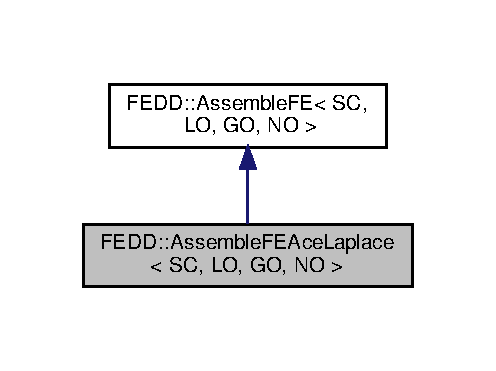
\includegraphics[width=238pt]{classFEDD_1_1AssembleFEAceLaplace__inherit__graph}
\end{center}
\end{figure}


Collaboration diagram for F\+E\+DD\+:\+:Assemble\+F\+E\+Ace\+Laplace$<$ SC, LO, GO, NO $>$\+:\nopagebreak
\begin{figure}[H]
\begin{center}
\leavevmode
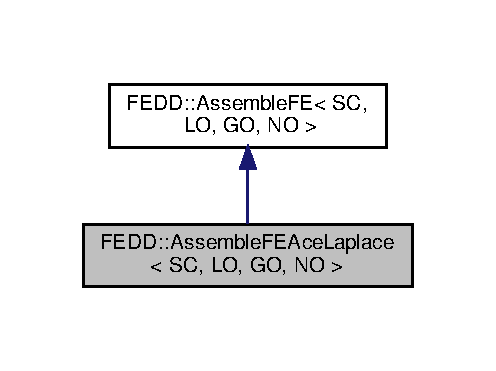
\includegraphics[width=238pt]{classFEDD_1_1AssembleFEAceLaplace__coll__graph}
\end{center}
\end{figure}
\subsection*{Public Types}
\begin{DoxyCompactItemize}
\item 
\mbox{\Hypertarget{classFEDD_1_1AssembleFEAceLaplace_ad5a1d233cdc46488449047924e868010}\label{classFEDD_1_1AssembleFEAceLaplace_ad5a1d233cdc46488449047924e868010}} 
typedef Matrix$<$ SC, LO, GO, NO $>$ {\bfseries Matrix\+\_\+\+Type}
\item 
\mbox{\Hypertarget{classFEDD_1_1AssembleFEAceLaplace_aef601b47321c72006e231340b6b79f01}\label{classFEDD_1_1AssembleFEAceLaplace_aef601b47321c72006e231340b6b79f01}} 
typedef Teuchos\+::\+R\+CP$<$ Matrix\+\_\+\+Type $>$ {\bfseries Matrix\+Ptr\+\_\+\+Type}
\item 
\mbox{\Hypertarget{classFEDD_1_1AssembleFEAceLaplace_aa8feabd583240a7d1dc1f826ac01bdff}\label{classFEDD_1_1AssembleFEAceLaplace_aa8feabd583240a7d1dc1f826ac01bdff}} 
typedef \hyperlink{classFEDD_1_1AssembleFE}{Assemble\+FE}$<$ SC, LO, GO, NO $>$ {\bfseries Assemble\+F\+E\+\_\+\+Type}
\end{DoxyCompactItemize}
\subsection*{Public Member Functions}
\begin{DoxyCompactItemize}
\item 
\hyperlink{classFEDD_1_1AssembleFEAceLaplace_a3e81060bb08ca1a1b9764e432eeed762}{Assemble\+F\+E\+Ace\+Laplace} (int flag, vec2\+D\+\_\+dbl\+\_\+\+Type nodes\+Ref\+Config, Parameter\+List\+Ptr\+\_\+\+Type parameters)
\begin{DoxyCompactList}\small\item\em Constructor for \hyperlink{classFEDD_1_1AssembleFEAceLaplace}{Assemble\+F\+E\+Ace\+Laplace}. \end{DoxyCompactList}\item 
virtual void \hyperlink{classFEDD_1_1AssembleFEAceLaplace_ab59722275fe6be6cdd4a1af48bd5a948}{assembly\+Laplacian} (Matrix\+Ptr\+\_\+\+Type \&element\+Matrix) const
\begin{DoxyCompactList}\small\item\em Assembly function for $ \int_T \nabla v \cdot \nabla u ~dx$. \end{DoxyCompactList}\item 
virtual void \hyperlink{classFEDD_1_1AssembleFEAceLaplace_af3ab42337c36c45446ecfa19bbb51134}{assembly\+R\+HS} (Vector\+Ptr\+\_\+\+Type \&element\+Vector) const
\begin{DoxyCompactList}\small\item\em Assembly function for $ \int_T f ~ v ~dx $, we need to. \end{DoxyCompactList}\end{DoxyCompactItemize}


\subsection{Constructor \& Destructor Documentation}
\mbox{\Hypertarget{classFEDD_1_1AssembleFEAceLaplace_a3e81060bb08ca1a1b9764e432eeed762}\label{classFEDD_1_1AssembleFEAceLaplace_a3e81060bb08ca1a1b9764e432eeed762}} 
\index{F\+E\+D\+D\+::\+Assemble\+F\+E\+Ace\+Laplace@{F\+E\+D\+D\+::\+Assemble\+F\+E\+Ace\+Laplace}!Assemble\+F\+E\+Ace\+Laplace@{Assemble\+F\+E\+Ace\+Laplace}}
\index{Assemble\+F\+E\+Ace\+Laplace@{Assemble\+F\+E\+Ace\+Laplace}!F\+E\+D\+D\+::\+Assemble\+F\+E\+Ace\+Laplace@{F\+E\+D\+D\+::\+Assemble\+F\+E\+Ace\+Laplace}}
\subsubsection{\texorpdfstring{Assemble\+F\+E\+Ace\+Laplace()}{AssembleFEAceLaplace()}}
{\footnotesize\ttfamily template$<$class SC , class LO , class GO , class NO $>$ \\
\hyperlink{classFEDD_1_1AssembleFEAceLaplace}{F\+E\+D\+D\+::\+Assemble\+F\+E\+Ace\+Laplace}$<$ SC, LO, GO, NO $>$\+::\hyperlink{classFEDD_1_1AssembleFEAceLaplace}{Assemble\+F\+E\+Ace\+Laplace} (\begin{DoxyParamCaption}\item[{int}]{flag,  }\item[{vec2\+D\+\_\+dbl\+\_\+\+Type}]{nodes\+Ref\+Config,  }\item[{Parameter\+List\+Ptr\+\_\+\+Type}]{params }\end{DoxyParamCaption})}



Constructor for \hyperlink{classFEDD_1_1AssembleFEAceLaplace}{Assemble\+F\+E\+Ace\+Laplace}. 


\begin{DoxyParams}[1]{Parameters}
\mbox{\tt in}  & {\em flag} & Flag of element \\
\hline
\mbox{\tt in}  & {\em nodes\+Ref\+Config} & Nodes of element in reference configuration \\
\hline
\mbox{\tt in}  & {\em params} & Parameterlist for current problem \\
\hline
\end{DoxyParams}


\subsection{Member Function Documentation}
\mbox{\Hypertarget{classFEDD_1_1AssembleFEAceLaplace_ab59722275fe6be6cdd4a1af48bd5a948}\label{classFEDD_1_1AssembleFEAceLaplace_ab59722275fe6be6cdd4a1af48bd5a948}} 
\index{F\+E\+D\+D\+::\+Assemble\+F\+E\+Ace\+Laplace@{F\+E\+D\+D\+::\+Assemble\+F\+E\+Ace\+Laplace}!assembly\+Laplacian@{assembly\+Laplacian}}
\index{assembly\+Laplacian@{assembly\+Laplacian}!F\+E\+D\+D\+::\+Assemble\+F\+E\+Ace\+Laplace@{F\+E\+D\+D\+::\+Assemble\+F\+E\+Ace\+Laplace}}
\subsubsection{\texorpdfstring{assembly\+Laplacian()}{assemblyLaplacian()}}
{\footnotesize\ttfamily template$<$class SC  = default\+\_\+sc, class LO  = default\+\_\+lo, class GO  = default\+\_\+go, class NO  = default\+\_\+no$>$ \\
void \hyperlink{classFEDD_1_1AssembleFEAceLaplace}{F\+E\+D\+D\+::\+Assemble\+F\+E\+Ace\+Laplace}$<$ SC, LO, GO, NO $>$\+::assembly\+Laplacian (\begin{DoxyParamCaption}\item[{Matrix\+Ptr\+\_\+\+Type \&}]{element\+Matrix }\end{DoxyParamCaption}) const\hspace{0.3cm}{\ttfamily [virtual]}}



Assembly function for $ \int_T \nabla v \cdot \nabla u ~dx$. 


\begin{DoxyParams}[1]{Parameters}
\mbox{\tt in}  & {\em \&element\+Matrix} & \\
\hline
\end{DoxyParams}
\mbox{\Hypertarget{classFEDD_1_1AssembleFEAceLaplace_af3ab42337c36c45446ecfa19bbb51134}\label{classFEDD_1_1AssembleFEAceLaplace_af3ab42337c36c45446ecfa19bbb51134}} 
\index{F\+E\+D\+D\+::\+Assemble\+F\+E\+Ace\+Laplace@{F\+E\+D\+D\+::\+Assemble\+F\+E\+Ace\+Laplace}!assembly\+R\+HS@{assembly\+R\+HS}}
\index{assembly\+R\+HS@{assembly\+R\+HS}!F\+E\+D\+D\+::\+Assemble\+F\+E\+Ace\+Laplace@{F\+E\+D\+D\+::\+Assemble\+F\+E\+Ace\+Laplace}}
\subsubsection{\texorpdfstring{assembly\+R\+H\+S()}{assemblyRHS()}}
{\footnotesize\ttfamily template$<$class SC  = default\+\_\+sc, class LO  = default\+\_\+lo, class GO  = default\+\_\+go, class NO  = default\+\_\+no$>$ \\
void \hyperlink{classFEDD_1_1AssembleFEAceLaplace}{F\+E\+D\+D\+::\+Assemble\+F\+E\+Ace\+Laplace}$<$ SC, LO, GO, NO $>$\+::assembly\+R\+HS (\begin{DoxyParamCaption}\item[{Vector\+Ptr\+\_\+\+Type \&}]{element\+Vector }\end{DoxyParamCaption}) const\hspace{0.3cm}{\ttfamily [virtual]}}



Assembly function for $ \int_T f ~ v ~dx $, we need to. 


\begin{DoxyParams}[1]{Parameters}
\mbox{\tt in}  & {\em \&element\+Vector} & \\
\hline
\end{DoxyParams}


The documentation for this class was generated from the following files\+:\begin{DoxyCompactItemize}
\item 
Assemble\+F\+E\+Ace\+Laplace\+\_\+decl.\+cpp\item 
Assemble\+F\+E\+Ace\+Laplace\+\_\+def.\+cpp\end{DoxyCompactItemize}

\hypertarget{classFEDD_1_1AssembleFEFactory}{}\section{F\+E\+DD\+:\+:Assemble\+F\+E\+Factory$<$ SC, LO, GO, NO $>$ Class Template Reference}
\label{classFEDD_1_1AssembleFEFactory}\index{F\+E\+D\+D\+::\+Assemble\+F\+E\+Factory$<$ S\+C, L\+O, G\+O, N\+O $>$@{F\+E\+D\+D\+::\+Assemble\+F\+E\+Factory$<$ S\+C, L\+O, G\+O, N\+O $>$}}
\subsection*{Public Types}
\begin{DoxyCompactItemize}
\item 
\mbox{\Hypertarget{classFEDD_1_1AssembleFEFactory_a42c8b5387f23fea233cb2c9b2bfc379f}\label{classFEDD_1_1AssembleFEFactory_a42c8b5387f23fea233cb2c9b2bfc379f}} 
typedef \hyperlink{classFEDD_1_1AssembleFE}{Assemble\+FE}$<$ SC, LO, GO, NO $>$ {\bfseries Assemble\+F\+E\+\_\+\+Type}
\item 
\mbox{\Hypertarget{classFEDD_1_1AssembleFEFactory_aa7e0143080c2d0fbe8df0d26c55d6b5c}\label{classFEDD_1_1AssembleFEFactory_aa7e0143080c2d0fbe8df0d26c55d6b5c}} 
typedef Teuchos\+::\+R\+CP$<$ \hyperlink{classFEDD_1_1AssembleFE}{Assemble\+F\+E\+\_\+\+Type} $>$ {\bfseries Assemble\+F\+E\+Ptr\+\_\+\+Type}
\end{DoxyCompactItemize}
\subsection*{Public Member Functions}
\begin{DoxyCompactItemize}
\item 
\mbox{\Hypertarget{classFEDD_1_1AssembleFEFactory_a29b1ce08865f9d32e7011e208a4cebb9}\label{classFEDD_1_1AssembleFEFactory_a29b1ce08865f9d32e7011e208a4cebb9}} 
\hyperlink{classFEDD_1_1AssembleFEFactory_a29b1ce08865f9d32e7011e208a4cebb9}{Assemble\+F\+E\+Factory} ()
\begin{DoxyCompactList}\small\item\em Constructor. \end{DoxyCompactList}\item 
Assemble\+F\+E\+Ptr\+\_\+\+Type \hyperlink{classFEDD_1_1AssembleFEFactory_a5f861160b72d42ff386b82be8e58604e}{build} (string problem\+Type, int flag, vec2\+D\+\_\+dbl\+\_\+\+Type nodes\+Ref\+Config, Parameter\+List\+Ptr\+\_\+\+Type params)
\begin{DoxyCompactList}\small\item\em We only need on function to build assemble\+FE, where we define the problem type and the \hyperlink{classFEDD_1_1AssembleFE}{Assemble\+FE} object we extend to a specific problem. \end{DoxyCompactList}\end{DoxyCompactItemize}


\subsection{Member Function Documentation}
\mbox{\Hypertarget{classFEDD_1_1AssembleFEFactory_a5f861160b72d42ff386b82be8e58604e}\label{classFEDD_1_1AssembleFEFactory_a5f861160b72d42ff386b82be8e58604e}} 
\index{F\+E\+D\+D\+::\+Assemble\+F\+E\+Factory@{F\+E\+D\+D\+::\+Assemble\+F\+E\+Factory}!build@{build}}
\index{build@{build}!F\+E\+D\+D\+::\+Assemble\+F\+E\+Factory@{F\+E\+D\+D\+::\+Assemble\+F\+E\+Factory}}
\subsubsection{\texorpdfstring{build()}{build()}}
{\footnotesize\ttfamily template$<$class SC , class LO , class GO , class NO $>$ \\
\hyperlink{classFEDD_1_1AssembleFEFactory}{Assemble\+F\+E\+Factory}$<$ SC, LO, GO, NO $>$\+::Assemble\+F\+E\+Ptr\+\_\+\+Type \hyperlink{classFEDD_1_1AssembleFEFactory}{F\+E\+D\+D\+::\+Assemble\+F\+E\+Factory}$<$ SC, LO, GO, NO $>$\+::build (\begin{DoxyParamCaption}\item[{string}]{problem\+Type,  }\item[{int}]{flag,  }\item[{vec2\+D\+\_\+dbl\+\_\+\+Type}]{nodes\+Ref\+Config,  }\item[{Parameter\+List\+Ptr\+\_\+\+Type}]{params }\end{DoxyParamCaption})}



We only need on function to build assemble\+FE, where we define the problem type and the \hyperlink{classFEDD_1_1AssembleFE}{Assemble\+FE} object we extend to a specific problem. 


\begin{DoxyParams}[1]{Parameters}
\mbox{\tt in}  & {\em problem\+Type} & Type of specfic problem we focus on \\
\hline
\mbox{\tt in}  & {\em flag} & Flag of element \\
\hline
\mbox{\tt in}  & {\em nodes\+Ref\+Config} & Nodes of element in reference configuration \\
\hline
\mbox{\tt in}  & {\em params} & Parameterlist for current problem \\
\hline
\end{DoxyParams}


The documentation for this class was generated from the following files\+:\begin{DoxyCompactItemize}
\item 
Assemble\+F\+E\+Factory\+\_\+decl.\+hpp\item 
Assemble\+F\+E\+Factory\+\_\+def.\+hpp\end{DoxyCompactItemize}

\hypertarget{classFEDD_1_1FE__Test}{}\section{F\+E\+DD\+:\+:F\+E\+\_\+\+Test$<$ SC, LO, GO, NO $>$ Class Template Reference}
\label{classFEDD_1_1FE__Test}\index{F\+E\+D\+D\+::\+F\+E\+\_\+\+Test$<$ S\+C, L\+O, G\+O, N\+O $>$@{F\+E\+D\+D\+::\+F\+E\+\_\+\+Test$<$ S\+C, L\+O, G\+O, N\+O $>$}}
\subsection*{Public Types}
\begin{DoxyCompactItemize}
\item 
\mbox{\Hypertarget{classFEDD_1_1FE__Test_a5e414af507a141db0961c32bf6b19825}\label{classFEDD_1_1FE__Test_a5e414af507a141db0961c32bf6b19825}} 
typedef Domain$<$ SC, LO, GO, NO $>$ {\bfseries Domain\+\_\+\+Type}
\item 
\mbox{\Hypertarget{classFEDD_1_1FE__Test_a1020475c408a64c7926feb8dded7f0c3}\label{classFEDD_1_1FE__Test_a1020475c408a64c7926feb8dded7f0c3}} 
typedef Teuchos\+::\+R\+CP$<$ Domain\+\_\+\+Type $>$ {\bfseries Domain\+Ptr\+\_\+\+Type}
\item 
\mbox{\Hypertarget{classFEDD_1_1FE__Test_a0a941851908a1e68d1554f8b28a7c72a}\label{classFEDD_1_1FE__Test_a0a941851908a1e68d1554f8b28a7c72a}} 
typedef Teuchos\+::\+R\+CP$<$ const Domain\+\_\+\+Type $>$ {\bfseries Domain\+Const\+Ptr\+\_\+\+Type}
\item 
\mbox{\Hypertarget{classFEDD_1_1FE__Test_a3345ab320c9e19d77dc7fec9645da0d0}\label{classFEDD_1_1FE__Test_a3345ab320c9e19d77dc7fec9645da0d0}} 
typedef std\+::vector$<$ Domain\+Const\+Ptr\+\_\+\+Type $>$ {\bfseries Domain\+Const\+Ptr\+\_\+vec\+\_\+\+Type}
\item 
\mbox{\Hypertarget{classFEDD_1_1FE__Test_a73f1a4ecb41cbeec1be473d71efe022d}\label{classFEDD_1_1FE__Test_a73f1a4ecb41cbeec1be473d71efe022d}} 
typedef Elements {\bfseries Elements\+\_\+\+Type}
\item 
\mbox{\Hypertarget{classFEDD_1_1FE__Test_af8f5bc3cb82c5d60a3a63b1e5c89a678}\label{classFEDD_1_1FE__Test_af8f5bc3cb82c5d60a3a63b1e5c89a678}} 
typedef Teuchos\+::\+R\+CP$<$ Elements\+\_\+\+Type $>$ {\bfseries Elements\+Ptr\+\_\+\+Type}
\item 
\mbox{\Hypertarget{classFEDD_1_1FE__Test_ab21a3d554ec8bf6763a7dabcbe800b35}\label{classFEDD_1_1FE__Test_ab21a3d554ec8bf6763a7dabcbe800b35}} 
typedef Matrix$<$ SC, LO, GO, NO $>$ {\bfseries Matrix\+\_\+\+Type}
\item 
\mbox{\Hypertarget{classFEDD_1_1FE__Test_a3c2e34afc3a1495c2b00313399f12b3d}\label{classFEDD_1_1FE__Test_a3c2e34afc3a1495c2b00313399f12b3d}} 
typedef Teuchos\+::\+R\+CP$<$ Matrix\+\_\+\+Type $>$ {\bfseries Matrix\+Ptr\+\_\+\+Type}
\item 
\mbox{\Hypertarget{classFEDD_1_1FE__Test_a11f3375e690a493e9076b63b0f86edf4}\label{classFEDD_1_1FE__Test_a11f3375e690a493e9076b63b0f86edf4}} 
typedef Small\+Matrix$<$ SC $>$ {\bfseries Small\+Matrix\+\_\+\+Type}
\item 
\mbox{\Hypertarget{classFEDD_1_1FE__Test_a675b52d9e58407c6baadb403394be92b}\label{classFEDD_1_1FE__Test_a675b52d9e58407c6baadb403394be92b}} 
typedef Teuchos\+::\+R\+CP$<$ Small\+Matrix\+\_\+\+Type $>$ {\bfseries Small\+Matrix\+Ptr\+\_\+\+Type}
\item 
\mbox{\Hypertarget{classFEDD_1_1FE__Test_a431ec5a97628feb8a0a8d16874ecd060}\label{classFEDD_1_1FE__Test_a431ec5a97628feb8a0a8d16874ecd060}} 
typedef Multi\+Vector$<$ SC, LO, GO, NO $>$ {\bfseries Multi\+Vector\+\_\+\+Type}
\item 
\mbox{\Hypertarget{classFEDD_1_1FE__Test_ac7c0363aa74e0bfcb903c13330c50185}\label{classFEDD_1_1FE__Test_ac7c0363aa74e0bfcb903c13330c50185}} 
typedef Teuchos\+::\+R\+CP$<$ Multi\+Vector\+\_\+\+Type $>$ {\bfseries Multi\+Vector\+Ptr\+\_\+\+Type}
\item 
\mbox{\Hypertarget{classFEDD_1_1FE__Test_afbc20c921480ce9f89ec045f94f6806a}\label{classFEDD_1_1FE__Test_afbc20c921480ce9f89ec045f94f6806a}} 
typedef \hyperlink{classFEDD_1_1AssembleFE}{Assemble\+FE}$<$ SC, LO, GO, NO $>$ {\bfseries Assemble\+F\+E\+\_\+\+Type}
\item 
\mbox{\Hypertarget{classFEDD_1_1FE__Test_a7a938cd88b5f936c58993fff97074e2d}\label{classFEDD_1_1FE__Test_a7a938cd88b5f936c58993fff97074e2d}} 
typedef Teuchos\+::\+R\+CP$<$ \hyperlink{classFEDD_1_1AssembleFE}{Assemble\+F\+E\+\_\+\+Type} $>$ {\bfseries Assemble\+F\+E\+Ptr\+\_\+\+Type}
\item 
\mbox{\Hypertarget{classFEDD_1_1FE__Test_a416d3abf702e778eb7fab3cd1feb3ede}\label{classFEDD_1_1FE__Test_a416d3abf702e778eb7fab3cd1feb3ede}} 
typedef Matrix\+\_\+\+Type\+::\+Map\+\_\+\+Type {\bfseries Map\+\_\+\+Type}
\item 
\mbox{\Hypertarget{classFEDD_1_1FE__Test_af41d3f3475a5ac2e0c7d3aab1b06102b}\label{classFEDD_1_1FE__Test_af41d3f3475a5ac2e0c7d3aab1b06102b}} 
typedef Matrix\+\_\+\+Type\+::\+Map\+Ptr\+\_\+\+Type {\bfseries Map\+Ptr\+\_\+\+Type}
\item 
\mbox{\Hypertarget{classFEDD_1_1FE__Test_ad09d94cdf8e7574fc9b6d1648fa18826}\label{classFEDD_1_1FE__Test_ad09d94cdf8e7574fc9b6d1648fa18826}} 
typedef Matrix\+\_\+\+Type\+::\+Map\+Const\+Ptr\+\_\+\+Type {\bfseries Map\+Const\+Ptr\+\_\+\+Type}
\item 
\mbox{\Hypertarget{classFEDD_1_1FE__Test_a1ac70a79e5935320b05ecf16739ad8a4}\label{classFEDD_1_1FE__Test_a1ac70a79e5935320b05ecf16739ad8a4}} 
typedef boost\+::function$<$ void(double $\ast$x, double $\ast$res, double t, const double $\ast$parameters)$>$ {\bfseries B\+C\+\_\+func\+\_\+\+Type}
\end{DoxyCompactItemize}
\subsection*{Public Member Functions}
\begin{DoxyCompactItemize}
\item 
\mbox{\Hypertarget{classFEDD_1_1FE__Test_a2e9a8640f2f6ed99376efbe84298e744}\label{classFEDD_1_1FE__Test_a2e9a8640f2f6ed99376efbe84298e744}} 
\hyperlink{classFEDD_1_1FE__Test_a2e9a8640f2f6ed99376efbe84298e744}{F\+E\+\_\+\+Test} (bool save\+Assembly=false)
\begin{DoxyCompactList}\small\item\em Constructor. \end{DoxyCompactList}\item 
void \hyperlink{classFEDD_1_1FE__Test_a9703f9144722f9c01e5bde489c2e6c2f}{add\+FE} (Domain\+Const\+Ptr\+\_\+\+Type domain)
\begin{DoxyCompactList}\small\item\em Adding underlying domains. \end{DoxyCompactList}\item 
void \hyperlink{classFEDD_1_1FE__Test_a1680db21378d38bdf239d64961497cb0}{assembly\+Laplace} (int dim, string F\+E\+Type, int degree, Matrix\+Ptr\+\_\+\+Type \&A, bool call\+Fill\+Complete=true, int F\+E\+Loc\+External=-\/1)
\begin{DoxyCompactList}\small\item\em Assembly of constant stiffness matix for laplacian operator $ \Delta $. \end{DoxyCompactList}\item 
void \hyperlink{classFEDD_1_1FE__Test_a262c614022e1bf4bf44cafb282494d15}{assembly\+R\+HS} (int dim, string F\+E\+Type, Multi\+Vector\+Ptr\+\_\+\+Type a, string field\+Type, Rhs\+Func\+\_\+\+Type func, vector$<$ SC $>$ \&func\+Parameter)
\begin{DoxyCompactList}\small\item\em Assembly of Rhs. \end{DoxyCompactList}\end{DoxyCompactItemize}
\subsection*{Public Attributes}
\begin{DoxyCompactItemize}
\item 
\mbox{\Hypertarget{classFEDD_1_1FE__Test_a9d4fe8878ab5ce8bf7817b2b7f57b1fc}\label{classFEDD_1_1FE__Test_a9d4fe8878ab5ce8bf7817b2b7f57b1fc}} 
bool {\bfseries save\+Assembly\+\_\+}
\item 
\mbox{\Hypertarget{classFEDD_1_1FE__Test_ad429d8e769350d7ab954942729d77674}\label{classFEDD_1_1FE__Test_ad429d8e769350d7ab954942729d77674}} 
Domain\+Const\+Ptr\+\_\+vec\+\_\+\+Type {\bfseries domain\+Vec\+\_\+}
\end{DoxyCompactItemize}


\subsection{Member Function Documentation}
\mbox{\Hypertarget{classFEDD_1_1FE__Test_a9703f9144722f9c01e5bde489c2e6c2f}\label{classFEDD_1_1FE__Test_a9703f9144722f9c01e5bde489c2e6c2f}} 
\index{F\+E\+D\+D\+::\+F\+E\+\_\+\+Test@{F\+E\+D\+D\+::\+F\+E\+\_\+\+Test}!add\+FE@{add\+FE}}
\index{add\+FE@{add\+FE}!F\+E\+D\+D\+::\+F\+E\+\_\+\+Test@{F\+E\+D\+D\+::\+F\+E\+\_\+\+Test}}
\subsubsection{\texorpdfstring{add\+F\+E()}{addFE()}}
{\footnotesize\ttfamily template$<$class SC , class LO , class GO , class NO $>$ \\
void \hyperlink{classFEDD_1_1FE__Test}{F\+E\+D\+D\+::\+F\+E\+\_\+\+Test}$<$ SC, LO, GO, NO $>$\+::add\+FE (\begin{DoxyParamCaption}\item[{Domain\+Const\+Ptr\+\_\+\+Type}]{domain }\end{DoxyParamCaption})}



Adding underlying domains. 


\begin{DoxyParams}[1]{Parameters}
\mbox{\tt in}  & {\em domain} & Finite element function space \\
\hline
\end{DoxyParams}
\mbox{\Hypertarget{classFEDD_1_1FE__Test_a1680db21378d38bdf239d64961497cb0}\label{classFEDD_1_1FE__Test_a1680db21378d38bdf239d64961497cb0}} 
\index{F\+E\+D\+D\+::\+F\+E\+\_\+\+Test@{F\+E\+D\+D\+::\+F\+E\+\_\+\+Test}!assembly\+Laplace@{assembly\+Laplace}}
\index{assembly\+Laplace@{assembly\+Laplace}!F\+E\+D\+D\+::\+F\+E\+\_\+\+Test@{F\+E\+D\+D\+::\+F\+E\+\_\+\+Test}}
\subsubsection{\texorpdfstring{assembly\+Laplace()}{assemblyLaplace()}}
{\footnotesize\ttfamily template$<$class SC , class LO , class GO , class NO $>$ \\
void \hyperlink{classFEDD_1_1FE__Test}{F\+E\+D\+D\+::\+F\+E\+\_\+\+Test}$<$ SC, LO, GO, NO $>$\+::assembly\+Laplace (\begin{DoxyParamCaption}\item[{int}]{dim,  }\item[{string}]{F\+E\+Type,  }\item[{int}]{degree,  }\item[{Matrix\+Ptr\+\_\+\+Type \&}]{A,  }\item[{bool}]{call\+Fill\+Complete = {\ttfamily true},  }\item[{int}]{F\+E\+Loc\+External = {\ttfamily -\/1} }\end{DoxyParamCaption})}



Assembly of constant stiffness matix for laplacian operator $ \Delta $. 


\begin{DoxyParams}[1]{Parameters}
\mbox{\tt in}  & {\em dim} & Dimension \\
\hline
\mbox{\tt in}  & {\em F\+E\+Type} & FE Discretization \\
\hline
\mbox{\tt in}  & {\em degree} & Degree of basis function \\
\hline
\mbox{\tt in}  & {\em A} & Resulting matrix \\
\hline
\mbox{\tt in}  & {\em call\+Fill\+Complete} & If Matrix A should be completely filled at end of function \\
\hline
\mbox{\tt in}  & {\em F\+E\+Loc\+External} & \\
\hline
\end{DoxyParams}
\mbox{\Hypertarget{classFEDD_1_1FE__Test_a262c614022e1bf4bf44cafb282494d15}\label{classFEDD_1_1FE__Test_a262c614022e1bf4bf44cafb282494d15}} 
\index{F\+E\+D\+D\+::\+F\+E\+\_\+\+Test@{F\+E\+D\+D\+::\+F\+E\+\_\+\+Test}!assembly\+R\+HS@{assembly\+R\+HS}}
\index{assembly\+R\+HS@{assembly\+R\+HS}!F\+E\+D\+D\+::\+F\+E\+\_\+\+Test@{F\+E\+D\+D\+::\+F\+E\+\_\+\+Test}}
\subsubsection{\texorpdfstring{assembly\+R\+H\+S()}{assemblyRHS()}}
{\footnotesize\ttfamily template$<$class SC , class LO , class GO , class NO $>$ \\
void \hyperlink{classFEDD_1_1FE__Test}{F\+E\+D\+D\+::\+F\+E\+\_\+\+Test}$<$ SC, LO, GO, NO $>$\+::assembly\+R\+HS (\begin{DoxyParamCaption}\item[{int}]{dim,  }\item[{string}]{F\+E\+Type,  }\item[{Multi\+Vector\+Ptr\+\_\+\+Type}]{a,  }\item[{string}]{field\+Type,  }\item[{Rhs\+Func\+\_\+\+Type}]{func,  }\item[{vector$<$ SC $>$ \&}]{func\+Parameter }\end{DoxyParamCaption})}



Assembly of Rhs. 


\begin{DoxyParams}[1]{Parameters}
\mbox{\tt in}  & {\em dim} & Dimension \\
\hline
\mbox{\tt in}  & {\em F\+E\+Type} & FE Discretization \\
\hline
\mbox{\tt in}  & {\em \&a} & Resulting vector \\
\hline
\mbox{\tt in}  & {\em field\+Type} & Vectorvalued or scalar rhs \\
\hline
\mbox{\tt in}  & {\em func} & Rhs function \\
\hline
\mbox{\tt in}  & {\em func\+Parameter} & Parameter for rhs function \\
\hline
\end{DoxyParams}


The documentation for this class was generated from the following files\+:\begin{DoxyCompactItemize}
\item 
Test\+F\+E/F\+E\+\_\+\+Test\+\_\+decl.\+hpp\item 
Test\+F\+E/F\+E\+\_\+\+Test\+\_\+def.\+hpp\end{DoxyCompactItemize}

%--- End generated contents ---

% Index
\backmatter
\newpage
\phantomsection
\clearemptydoublepage
\addcontentsline{toc}{chapter}{Index}
\printindex

\end{document}
